\subsection{CHANGE OF BASES}

PROPOSITION 4. Let E be a right A-module with finite basis \((e_i)_{1 \leqslant i \leqslant n}\) of \(n\) elements.

For a family of \(n\) elements \(e_i' = \sum_{j=1} e_j a_{ji} (1 \leqslant i \leqslant n)\) to be a basis of \(\mathbf{E}\) , it is necessary and sufficient that the square matrix \(P = (a_{ji})\) of order \(n\) be invertible.

P is just the matrix, with respect to the basis \((e_{i})\) of the endomorphism u of E defined by \(u(e_{i}) = e_{i}^{\prime} (1 \leqslant i \leqslant n)\) . Now, for u to be an automorphism of E, it is necessary and sufficient that \((u(e_{i}))\) be a basis of E (§ 1, no. 11, Corollary 3 to Proposition 17); whence the proposition.

The invertible matrix P is called the matrix of passage from the basis \((e_{i})\) to the basis \((e_{i}^{\prime})\) . It can also be interpreted as the matrix of the identity mapping \(1_{E}\) with respect to the bases \((e_{i}^{\prime})\) and \((e_{i})\) (in that order); then clearly the matrix of passage from the basis \((e_{i}^{\prime})\) to the basis \((e_{i})\) is the inverse \(P^{-1}\) of P.

PROPOSITION 5. Let \((e_i)\) , \((e_i')\) be two bases of \(n\) elements of \(\mathbf{E}\) and \(P\) the matrix of passage from \((e_i)\) to \((e_i')\) . If \((e_i^*)\) and \((e_i'^*)\) are the respective dual bases of \((e_i)\) and \((e_i')\) , the matrix of passage from \((e_i^*)\) to \((e_i'^*)\) is the contragredient \(^t P^{-1}\) of \(P\) .

The transpose of the identity mapping \(1_{E}\) is the identity mapping \(1_{E^{*}}\) ; by Proposition 3, no. 4, the matrix of \(1_{E^{*}}\) with respect to the bases \((e_{i}^{\prime*})\) and \((e_{i}^{*})\) (in that order) is the transpose of the matrix of \(1_{E}\) with respect to the bases \((e_{i})\) and \((e_{i}^{\prime})\) (in that order), that is the transpose of \(P^{-1}\) .

PROPOSITION 6. Let E and F be two right A-modules, \((e_i)\) and \((e_i')\) two bases of E with \(n\) elements, \((f_j)\) and \((f_j')\) two bases of \(F\) with \(m\) elements, \(P\) the matrix of passage from \((e_i)\) to \((e_i')\) and \(Q\) the matrix of passage from \((f_j)\) to \((f_j')\) . For every linear mapping \(u\) of \(E\) into \(F\) , let \(M(u)\) be the matrix of \(u\) with respect to the bases \((e_i)\) and \((f_j)\) and \(M'(u)\) the matrix of \(u\) with respect to the bases \((e_i')\) and \((f_i')\) ; then

\[
M ^ {\prime} (u) = Q ^ {- 1} M (u) P.\tag{33 D}
\]

We may write \(u = 1_{\mathbb{F}} \circ u \circ 1_{\mathbb{E}}\) . Formula (33) follows immediately from no. 4, Corollary to Proposition 2 when the matrix of \(1_{\mathbb{E}}\) is taken with respect to \((e_i')\) and \((e_i)\) , that of \(u\) with respect to \((e_i)\) and \((f_i)\) and that of \(1_{\mathbb{F}}\) with respect to \((f_i)\) and \((f_j')\) .

COROLLARY 1. If \(u\) is an endomorphism of \(E\) and \(M(u)\) and \(M'(u)\) its matrices with respect to the bases \((e_1)\) and \((e_1')\) respectively, then

\[
M ^ {\prime} (u) = P ^ {- 1} M (u) P.\tag{34 D}
\]

COROLLARY 2. If \(M(x)\) and \(M'(x)\) are the matrices with one column of the same element \(x \in E\) with respect to the bases \((e_i)\) and \((e_i')\) respectively, then

\[
M (x) = P. M ^ {\prime} (x).\tag{35 D}
\]

This is a special case of Proposition 6, applied to the mapping \(\theta_{x}:a\mapsto xa\) of \(\mathbf{A}_d\) to \(\mathbf{E}\) (no. 4, Remark 1).

Formula (35) is equivalent to

\[
x _ {i} = \sum_ {j = 1} ^ {n} a _ {i j} x _ {j} ^ {\prime} (1 \leqslant i \leqslant n)\tag{36 D}
\]

for the elements \(x_{i}\) and \(x_{i}^{\prime}\) of the matrices \(M(x)\) and \(M^{\prime}(x)\) respectively. Formulae (36 D) are called formulae of change of coordinates. Observe that they express the components of x relative to the ``old'' basis ( \(e_{i}\) ) as functions of the components of x relative to the ``new'' basis ( \(e_{i}^{\prime}\) ) and the elements of P, that is the components of the ``new'' basis relative to the ``old'' basis.

Remarks. (1) We now start with a left A-module E with two bases \((e_{i})\) , \((e_{i}^{\prime})\) , each with n elements; if we write \(e_{i}^{\prime} = \sum_{j=1}^{n} a_{ji} e_{i}\) , \(P = (a_{ji})\) is also called the matrix of passing from \((e_{i})\) to \((e_{i}^{\prime})\) ; it is also the matrix of the automorphism of E such that \(u(e_{i}) = e_{i}^{\prime}\) , with respect to the basis \((e_{i})\) and also the matrix of \(1_{E}\) with respect to the bases \((e_{i}^{\prime})\) and \((e_{i})\) in that order. The above results then hold with only the following modifications: formulae (33 D) to (36 D) are respectively replaced by

\[
{ } ^ { t } M ^ { \prime } ( u ) = { } ^ { t } P . { } ^ { t } M ( u ) . { } ^ { t } Q ^ { - 1 }\tag{33 G}
\]

\[
{ } ^ { t } M ^ { \prime } ( u ) = { } ^ { t } P . { } ^ { t } M ( u ) . { } ^ { t } P ^ { - 1 }\tag{34 G}
\]

\[
{ } ^ { t } M ( u ) = { } ^ { t } M ^ { \prime } ( u ) . { } ^ { t } P .\tag{35 G}
\]

\[
\kappa_ {i} = \sum_ {j = 1} ^ {n} x _ {j} ^ {\prime} a _ {i j} \quad (1 \leqslant i \leqslant n).\tag{36 G}
\]

\begin{enumerate}
\def\labelenumi{(\arabic{enumi})}
\setcounter{enumi}{1}
\tightlist
\item
  Under the hypotheses of Proposition 4, consider an element \(x^{*} \in \mathbf{E}^{*}\) ; as the matrix of passage from \((e_i^*)\) to \((e_i'^*)\) is \(^tP^{-1}\) (Proposition 5), for the matrices \(M(x^{*})\) and \(M'(x^{*})\) of \(x^{*}\) with respect to these two bases respectively,
\end{enumerate}

\[
{ } ^ { t } M ( x ^ { * } ) = { } ^ { t } M ^ { \prime } ( x ^ { * } ) . P ^ { - 1 }
\]

or also

\[
{ } ^ { t } M ^ { \prime } ( x ^ { * } ) = { } ^ { t } M ( x ^ { * } ) . P\tag{37 D}
\]

which is equivalent to the system of equations

\[
x _ {i} ^ {\prime *} = \sum_ {j = 1} ^ {n} x _ {j} ^ {*} a _ {j i} (1 \leqslant i \leqslant n)\tag{38 D}
\]

for the elements \((x_{i}^{*})\) and \((x_{i}^{\prime *})\) of the matrices \(M(x^{*})\) and \(M'(x^{*})\) . The corresponding formulae for a left A-module E are

\[
M ^ {\prime} (x ^ {*}) = ^ {t} P. M (x ^ {*})\tag{37 G}
\]

\[
x _ {i} ^ {\prime *} = \sum_ {j = 1} ^ {n} a _ {j i} x _ {j} ^ {*} (1 \leqslant i \leqslant n).\tag{38 G}
\]

\begin{enumerate}
\def\labelenumi{(\arabic{enumi})}
\setcounter{enumi}{2}
\tightlist
\item
  Let A, B be two rings, \(\sigma: \mathbf{A} \to \mathbf{B}\) a homomorphism of A into B, E a right (resp. left) A-module, \((e_i)\) , \((e_i')\) two bases with \(n\) elements of E, F a right (resp. left) B-module, \((f_j)\) , \((f_j')\) two bases with \(m\) elements of F and \(P\) (resp. \(Q\) ) the matrix of passage from \((e_i)\) to \((e_i')\) (resp. from \((f_j)\) to \((f_j')\) ).
\end{enumerate}

For every semi-linear mapping \(u: \mathbf{E} \to \mathbf{F}\) , relative to \(\sigma\) , let \(M(u)\) be the matrix of \(u\) with respect to \((e_i)\) and \((f_j)\) and \(M'(u)\) its matrix with respect to \((e_i')\) and \((f_j')\) . Then

\[
M ^ {\prime} (u) = Q ^ {- 1} M (u) \sigma (P)\tag{39 D}
\]

(resp.

\[
{ } ^ { t } M ^ { \prime } ( u ) = \sigma ( { } ^ { t } P ) . { } ^ { t } M ( u ) . { } ^ { t } Q ^ { - 1 } ) .\tag{39 G}
\]

The proof is the same as that for (33 D) and (33 G), this time using formulae (27 D) and (27 G) (no. 6).

\subsection{EQUIVALENT MATRICES; SIMILAR MATRICES}

DEFINITION 5. Two matrices \(X, X'\) with \(m\) rows and \(n\) columns over a ring are called equivalent if there exists an invertible square matrix \(P\) of order \(m\) and an invertible square matrix \(Q\) of order \(n\) such that

\[
X ^ {\prime} = P X Q.\tag{40}
\]

Clearly the relation ``X and \(X'\) are equivalent'' is an equivalence relation (Set Theory, II, § 6, no. 1) on the set \(A^{mn}\) of matrices of type \((m, n)\) over A, which justifies the terminology.

With this definition, Proposition 6 of no. 8 can be stated by saying that when the bases are changed in two right A-modules E, F (with finite bases), the matrix of a linear mapping \(u \colon \mathbf{E} \to \mathbf{F}\) with respect to the new bases is equivalent to the matrix of \(u\) with respect to the old bases.

Conversely, if relation (40) holds and \(u \colon \mathbf{A}_d^n \to \mathbf{A}_d^m\) is a linear mapping whose matrix is \(X\) with respect to the respective canonical bases \((e_i)\) and \((f_j)\) of \(\mathbf{A}_d^n\) and \(\mathbf{A}_d^m\) , then \(X'\) is the matrix of \(u\) with respect to the bases \((e_i')\) and \((f_j')\) such that \(Q\) is the matrix of passage from \((e_i)\) to \((e_i')\) and \(P^{-1}\) the matrix of passage from \((f_j)\) to \((f_j')\) .

Examples of equivalent matrices. (1) Two matrices \(X = (x_{ij})\) and \(X' = (x_{ij}')\) with \(m\) rows and \(n\) columns ``differ only in the order of their rows'' if there exists a permutation \(\sigma\) of the interval \([1, m]\) of \(\mathbf{N}\) , such that for every ordered pair of indices \((i,j)\) , \(x_{ij}' = x_{\sigma(i),j}\) (we also say that \(X'\) is obtained by performing the permutation \(\sigma^{-1}\) on the rows of \(X\) ). The matrices \(X\) and \(X'\) are then equivalent, for \(X' = PX\) , where \(P\) is the matrix of the permutation \(\sigma^{-1}\) (cf.~no. 7, Example II).

Similarly X and \(X'\) are said to differ only in the order of their columns if there exists a permutation \(\tau\) of \([1, n]\) such that \(x_{ij}' = x_{i,\tau(j)}\) for every ordered pair of indices \((i,j)\) , X and \(X'\) are also equivalent, for \(X' = XQ\) where Q is the matrix of the permutation \(\tau\) .

Note that in the above notation \(P\) is the matrix of passage from a basis \((f_j)_{1 \leqslant j \leqslant m}\) to the basis \((f_\sigma^{-1}(j))_{1 \leqslant j \leqslant m}\) and \(Q\) the matrix of passage from a basis \((e_i)_{1 \leqslant i \leqslant n}\) to the basis \((e_{\tau(i)})_{1 \leqslant i \leqslant n}\) .

\begin{enumerate}
\def\labelenumi{(\arabic{enumi})}
\setcounter{enumi}{1}
\tightlist
\item
  Let \(j, k\) be distinct elements of \([1, n]\) and let \(a \in A\) .
\end{enumerate}

Suppose that for \(1 \leqslant i \leqslant m\) , \(x_{ij}' = x_{ij} + x_{ik}a\) and \(x_{il}' = x_{il}\) for \(j \neq l\) and \(1 \leqslant i \leqslant m\) ; \(X'\) is said to be derived from \(X\) by adding to the column of \(X\) of index \(j\) the column of index \(k\) multiplied on the right by \(a\) . In this case \(X\) and \(X'\) are also equivalent: for if \(Q = I_n + aE_{kj}\) (an invertible triangular matrix, as seen in no. 7), then \(X' = XQ\) .

Similarly, let \(h, i\) be two distinct elements of \([1, m]\) and \(a\) an element of \(A\) ; if \(X'\) is derived from \(X\) by adding to the row of \(X\) of index \(i\) the row of index \(h\) multiplied on the left by \(a, X\) and \(X'\) are equivalent, for \(X' = PX\) , where \(P = I_m + aE_{th}\) .

\begin{enumerate}
\def\labelenumi{(\arabic{enumi})}
\setcounter{enumi}{2}
\tightlist
\item
  Finally, if, for a given index \(j\) , \(x_{ij}' = x_{ij}c\) for \(1 \leqslant i \leqslant m\) , where \(c\) is invertible and \(x_{il}' = x_{il}\) for \(1 \leqslant i \leqslant m\) and \(l \neq j\) , \(X\) and \(X'\) are equivalent; for \(X' = XQ\) , where \(Q\) is the matrix \(\text{diag}(a_k)\) with \(a_j = c\) , \(a_k = 1\) for \(k \neq j\) . Then \(X'\) is said to be derived from \(X\) by multiplying the column of \(X\) of index \(j\) on the right by \(a\) .
\end{enumerate}

Similarly, if \(X'\) is derived from \(X'\) by multiplying the row of \(X\) of index \(i\) on the left by an invertible element \(c \in A\) , \(X'\) and \(X\) are equivalent, for \(X' = PX\) where \(P\) is the matrix \(\text{diag}(b_h)\) with \(b_i = c\) , \(b_h = 1\) for \(h \neq i\) .

DEFINITION 6. Two square matrices \(X, X'\) of order \(n\) over a ring \(A\) are called similar if there exists an invertible square matrix \(P\) of order \(n\) such that

\[
X ^ {\prime} = P X P ^ {- 1}\tag{41}
\]

Clearly the relation ``X and \(X'\) are similar'' is an equivalence relation on \(\mathbf{M}_{n}(\mathbf{A})\) meaning that X and \(X'\) are transformed into one another by an inner automorphism of this ring.

With this definition, Corollary 1 to Proposition 6 of no. 8 can be stated by saying that when the basis of an A-module E (with a finite basis) is changed, the matrix of an endomorphism u with respect to the new basis is similar to the matrix of u with respect to the old basis.

Remarks. (1) Two square matrices which differ only in the order of their rows (or the order of their columns) are equivalent, but in general not similar. A matrix similar to a square matrix \(X = (x_{ij})\) can be obtained by performing the same permutation \(\sigma^{-1}\) on the rows and columns, that is by considering the matrix \(X' = (x_{ij}')\) , where \(x_{ij}' = x_{\sigma(i),\sigma(j)}\) for every ordered pair of indices; for if \(X\) is the matrix of an endomorphism \(u\) of \(A_d^n\) with respect to a basis \((e_i)_{1 \leq i \leq n}\) , \(X'\) is the matrix of \(u\) with respect to the basis \((e_{\sigma(i)})_{1 \leq i \leq n}\) .

\begin{enumerate}
\def\labelenumi{(\arabic{enumi})}
\setcounter{enumi}{1}
\tightlist
\item
  Let \(X\) and \(X'\) be two square matrices of order \(n\) which can be written in the form of diagonal matrices of square matrices (no. 7, Example IV):
\end{enumerate}

\[
X = \left( \begin{array}{c c c c} X _ {1} & 0 & \ldots & 0 \\ 0 & X _ {2} & \ldots & 0 \\ \cdot & \cdot & \cdot & \cdot \\ 0 & 0 & \ldots & X _ {p} \end{array} \right) \qquad X ^ {\prime} = \left( \begin{array}{c c c c} X _ {1} ^ {\prime} & 0 & \ldots & 0 \\ 0 & X _ {2} ^ {\prime} & \ldots & 0 \\ \cdot & \cdot & \cdot & \cdot \\ 0 & 0 & \ldots & X _ {p} ^ {\prime} \end{array} \right)
\]

corresponding to the same partition of the indexing set \([1, n]\) for X and \(X'\) . If, for \(1 \leqslant i \leqslant p\) , \(X_i\) and \(X'_i\) are equivalent (resp. similar), then X and \(X'\) are equivalent (resp. similar): for, if \(X'_i = P_i X_i Q_i\) for \(1 \leqslant i \leqslant p\) , then \(X' = PXQ\) where

\[
P = \left( \begin{array}{c c c c c} P _ {1} & 0 & \dots & 0 \\ 0 & P _ {2} & \dots & 0 \\ \cdot & \cdot & \cdot & \cdot & \cdot \\ 0 & 0 & \dots & P _ {p} \end{array} \right) \quad Q = \left( \begin{array}{c c c c c} Q _ {1} & 0 & \dots & 0 \\ 0 & Q _ {2} & \dots & 0 \\ \cdot & \cdot & \cdot & \cdot & \cdot \\ 0 & 0 & \dots & Q _ {p} \end{array} \right)
\]

as follows from calculating the ``block'' product (no. 6). Moreover, if \(Q_{i} = P_{i}^{-1}\) for all i, then \(Q = P^{-1}\) .

\subsection{TENSOR PRODUCT OF MATRICES OVER A COMMUTATIVE RING}

Let C be a commutative ring, E, F, U, V four C-modules and \(\phi:E\to U\) , \(\psi:F\to V\) two C-linear mappings. Suppose that E, F, U, V have respectively finite bases \((e_{\lambda})_{\lambda \in L}, (f_{\mu})_{\mu \in M}, (u_{\rho})_{\rho \in R}, (v_{\sigma})_{\sigma \in S}\) ; let \(A = (a_{\rho \lambda})\) be the matrix of \(\phi\) with respect to \((e_{\lambda})\) and \((u_{\rho})\) , \(B = (b_{\sigma \mu})\) that of \(\psi\) with respect to \((f_{\mu})\) and \((v_{\sigma})\) . For every ordered pair \((\lambda, \mu) \in L \times M = N\) , let \(g_{\lambda \mu} = e_{\lambda} \otimes f_{\mu}\) ; for every ordered pair \((\rho, \sigma) \in R \times S = T\) let \(w_{\rho \sigma} = u_{\rho} \otimes v_{\sigma}\) ; the \(g_{\lambda \mu}\) then form a basis of \(E \otimes F\) and the \(w_{\rho \sigma}\) a basis of \(U \otimes V\) ( \(\S 3\) , no. 6, Corollary 2 to Proposition 7). The tensor product of \(A\) by \(B\) , denoted by \(A \otimes B\) , is the matrix \(X = (x_{\tau v})(\tau, v) \in T \times N\) whose elements are given by

\[
x _ {(\rho , \sigma), (\lambda , \mu)} = a _ {\rho \lambda} b _ {\sigma \mu}.\tag{42}
\]

Then \(A \otimes B\) is the matrix of \(\phi \otimes \psi\) with respect to the bases \((g_{\lambda \mu})\) and \((w_{\rho \sigma})\) . By definition (§ 3, no. 2, formula (3))

\[
\begin{array}{r l} (\phi \otimes \psi) (g _ {\lambda \mu}) & = (\phi \otimes \psi) (e _ {\lambda} \otimes f _ {\mu}) = \phi (e _ {\lambda}) \otimes \psi (f _ {\mu}) \\ & = \sum_ {\rho , \sigma} a _ {\rho \lambda} b _ {\sigma \mu} (u _ {\rho} \otimes v _ {\sigma}) = \sum_ {\rho , \sigma} a _ {\rho \lambda} b _ {\sigma \mu} w _ {\rho \sigma}. \end{array}
\]

Definition (42) of the elements of \(A \otimes B\) shows that this matrix corresponds bijectively with the matrix of matrices \((a_{\rho \lambda}B)_{(\rho, \lambda) \in \mathbb{R} \times \mathbb{L}}\) and also the matrix \((Ab_{\sigma \mu})_{(\sigma, \mu) \in \mathbb{S} \times \mathbb{M}}\) (no. 5).

The fact that \((\phi, \psi) \mapsto \phi \otimes \psi\) is a C-bilinear mapping and formula (9) of §3, no. 5, can be expressed by the identities

\[
\left\{ \begin{array}{l} A \otimes (B _ {1} + B _ {2}) = A \otimes B _ {1} + A \otimes B _ {2} \\ (A _ {1} + A _ {2}) \otimes B = A _ {1} \otimes B + A _ {2} \otimes B \end{array} \right.\tag{43}
\]

\[
(c A) \otimes B = A \otimes (c B) = c (A \otimes B) \quad \text { for } c \in \mathbf {C}\tag{44}
\]

\[
(A _ {1} \otimes B _ {1}) (A _ {2} \otimes B _ {2}) = (A _ {1} A _ {2}) \otimes (B _ {1} B _ {2})\tag{45}
\]

when the operations appearing are defined. The transpose of a tensor product of matrices is given by

\[
{ } ^ { t } ( A \otimes B ) = ( { } ^ { t } A ) \otimes ( { } ^ { t } B ) .\tag{46}
\]

If A and B are invertible square matrices over C, \(A \otimes B\) is invertible and

\[
(A \otimes B) ^ {- 1} = (A ^ {- 1}) \otimes (B ^ {- 1}).\tag{47}
\]

Let \((e_{\lambda}^{\prime})_{\lambda \in L}\) be another basis of E and \((f_{\mu}^{\prime})_{\mu \in M}\) another basis of F; if P is the matrix of passage from the basis \((e_{\lambda})\) to the basis \((e_{\lambda}^{\prime})\) and Q the matrix of passage from the basis \((f_{\mu})\) to the basis \((f_{\mu}^{\prime})\) , the matrix of passage from the basis \((e_{\lambda} \otimes f_{\mu})\) to the basis \((e_{\lambda}^{\prime} \otimes f_{\mu}^{\prime})\) is \(P \otimes Q\) . If \(A^{\prime}\) is equivalent (resp. similar) to A and \(B^{\prime}\) equivalent (resp. similar) to B, then \(A^{\prime} \otimes B^{\prime}\) is equivalent (resp. similar) to \(A \otimes B\) .

The definition of tensor product of matrices can be generalized in an obvious way to an arbitrary finite number of matrices over C; in particular we have the associativity formula

\[
\left(\bigotimes_ {i \in I _ {1}} X _ {i}\right) \otimes \left(\bigotimes_ {i \in I _ {2}} X _ {i}\right) = \bigotimes_ {i \in I} X _ {i}\tag{48}
\]

for every partition \((\mathbf{I}_{1}, \mathbf{I}_{2})\) of the finite indexing set I.

\subsection{TRACE OF A MATRIX}

Let C be a commutative ring; for every square matrix \(X = (x_{ij})\) over C corresponding to the finite indexing set I, the trace of X is the element

\[
\operatorname{Tr} (X) = \sum_ {i \in I} x _ {i i}.\tag{49}
\]

Let E be a C-module admitting a finite basis \((e_{i})_{i\in I}\) ; for every endomorphism u of E,

\[
\operatorname{Tr} (u) = \operatorname{Tr} (M (u))\tag{50}
\]

\(M(u)\) being the matrix u with respect to the basis \((e_{i})\) ; this follows immediately from § 4, no. 3, formula (17), when this formula is applied to the endomorphism \(x \mapsto \langle x, e_{i}^{*} \rangle e_{j}\) (where \(e_{i}^{*}\) ) is the dual basis of \((e_{i})\) ); from this we pass to the general case by linearity. Formula (49) shows that

\[
\operatorname{Tr} (u) = \sum_ {i} \left\langle u (e _ {i}), e _ {i} ^ {*} \right\rangle\tag{51}
\]

for every basis \((e_i)\) of E (cf.~§4, no. 3, formula (17)).

If X is a matrix of type \((m, n)\) over C and Y a matrix of type \((n, m)\) over C, then

\[
\operatorname{Tr} (X Y) = \operatorname{Tr} (Y X)\tag{52}
\]

as follows from the above and Proposition 3 of § 4, no. 3; (52) can also be obtained directly, for if \(X = (x_{ij})\) , \(Y = (y_{ji})\) ( \(1 \leqslant i \leqslant m\) , \(1 \leqslant j \leqslant n\) ), then

\[
\operatorname{Tr} (X Y) = \sum_ {i, j} x _ {i j} y _ {j i}\tag{53}
\]

by (49). The latter formula proves moreover:

PROPOSITION 7. Let C be a commutative ring and for every matrix \(P \in \mathbf{M}_n(\mathbf{C})\) let \(f_P\) be the linear form \(X \mapsto \operatorname{Tr}(PX)\) on \(\mathbf{M}_n(\mathbf{C})\) ; the mapping \(P \mapsto f_P\) is a C-linear bijection of \(\mathbf{M}_n(\mathbf{C})\) onto its dual.

PROPOSITION 8. If \(g\) is a linear form on the C-module \(\mathbf{M}_n(\mathbf{C})\) such that \(g(XY) = g(YX)\) for all matrices \(X, Y\) in \(\mathbf{M}_n(\mathbf{C})\) , there exists one and only one scalar \(c \in \mathbf{C}\) such that \(g(X) = c\) . Tr(X) for every matrix \(X \in \mathbf{M}_n(\mathbf{C})\) .

Since the proposition is trivial for \(n = 1\) , attention may be confined to the case where \(n \geqslant 2\) . Taking \(X = E_{ij}\) , \(Y = E_{jk}\) with \(i \neq k\) , we obtain \(g(E_{ik}) = 0\) ; then taking \(X = E_{ij}\) , \(Y = E_{ji}\) with \(i \neq j\) , we find \(g(E_{ii}) = g(E_{jj})\) ; the proposition follows immediately since the \(E_{ij}\) form a basis of \(\mathbf{M}_n(\mathbf{C})\) .

\subsection{MATRICES OVER A FIELD}

The finite matrices with m rows and n columns over a field K are in one-to-one correspondence with the linear mappings of the right vector space \(E = K_{d}^{n}\) into the right vector space \(K_{d}^{m}\) when the matrices of these mappings are taken with respect to the canonical bases of E and F. By definition, the rank of such a matrix X is the rank of the linear mapping \(u: E \to F\) corresponding to it; as this number is by definition the dimension of the subspace \(u(E)\) of F, it amounts to the same (identifying the columns of X with the images under u of the canonical basis of E) to give the following definition:

DEFINITION 7. Given a matrix X with m rows and n columns over a field K, the dimension of the subspace of \(K_{d}^{m}\) generated by the n columns of X is called the rank of X with respect to K and denoted by \(\operatorname{rg}(X)\) .

It can also be said that the rank of X is the maximum number of linearly independent columns of X (as elements of \(K_{d}^{m}\) ). Obviously \(\operatorname{rg}(X) \leqslant \inf(m, n)\) ; for every submatrix Y of X, \(\operatorname{rg}(Y) \leqslant \operatorname{rg}(X)\) .

If E and F are two finite-dimensional vector spaces over K and u a linear mapping of E into F, the rank of the matrix \(M(u)\) with respect to any two bases is equal to the rank of u.

PROPOSITION 9. If the elements of a matrix X with m rows and n columns belong to a subfield \(K_{0}\) of a field K, the rank of X with respect to \(K_{0}\) is equal to the rank of X with respect to K.

Let \(F_{0}\) be the right vector \(K_{0}\) -space generated by the canonical basis of the right vector K-space \(E = K_{d}^{m}\) ; by hypothesis the columns of X belong to \(E_{0}\) . Let \(V_{0}\) (resp. V) be the vector sub- \(K_{0}\) -space of \(F_{0}\) (resp. the vector sub-K-space of E) generated by these columns. Then \(V = V_{0} \otimes_{K_{0}} K\) (§ 8, no. 2, Proposition 2) and hence \(\dim_{K} V = \dim_{K_{0}} V_{0}\) .

PROPOSITION 10. The rank of a matrix X over a field K is equal to the rank of its transpose \(^{t}X\) over the opposite field \(K^{0}\) .

In the notation introduced before Definition 7, the rank of u is equal to that of \({}^{t}u\) (§ 7, no. 5, Proposition 10) and the proposition therefore follows from no. 4, Proposition 3.

It is thus seen that the rank of X can also be defined as the maximum number of linearly independent rows of X (considering them as elements of the left vector K-space \(K_{s}^{n}\) ).

The square matrices of order n over a field K correspond bijectively with the endomorphisms of \(E = K_{d}^{n}\) and form a ring isomorphic to the ring

End \(_{\kappa}\) (E) (no. 7); corresponding to the automorphisms of E are the invertible square matrices.

PROPOSITION 11. Let \(X\) be a square matrix of order \(n\) over a field \(K\) . The following properties are equivalent:

\begin{enumerate}
\def\labelenumi{(\alph{enumi})}
\item
  \(X\) is invertible in \(\mathbf{M}_n(\mathbf{K})\) .
\item
  \(X\) is right invertible in \(\mathbf{M}_n(\mathbf{K})\) .
\item
  \(X\) is left invertible in \(\mathbf{M}_n(\mathbf{K})\) .
\item
  \(X\) is of rank \(n\) .
\end{enumerate}

This is just a translation of § 7, no. 4, Corollary to Proposition 9.

PROPOSITION 12. For a system of \(m\) linear equations in \(n\) unknowns

\[
\sum_ {j = 1} ^ {n} a _ {i j} x _ {j} = b _ {i} \quad (1 \leqslant i \leqslant m)\tag{54}
\]

over a field K to have at least one solution, it is necessary and sufficient that the matrix \(A = (a_{ij})\) of the system and the matrix B, obtained by bordering A with an \((n + 1)\) -th column equal to \((b_{i})\) , be matrices of the same rank.

It has been seen (no. 4) that the existence of a solution of (54) is equivalent to the fact that the column \((b_{i})\) is a linear combination of the columns of A and the proposition therefore follows from §7, no. 3, Corollary 4 to Proposition 4.

Note that the condition of Proposition 12 is always fulfilled when m = n and A is invertible, that is of rank n (Proposition 11). If x and b then denote the matrices with one column \((x_{i})\) and \((b_{i})\) respectively, system (54) is equivalent to A. x = b and its unique solution is \(x = A^{-1}.b\) .

\subsection{EQUIVALENCE OF MATRICES OVER A FIELD}

PROPOSITION 13. Let E, F be two finite-dimensional vector spaces over a field K. If \(u: \mathbf{E} \to \mathbf{F}\) is a linear mapping of rank \(r\) , there exist bases of E and F such that, with respect to these bases,

\[
M (u) = \left( \begin{array}{c c} I _ {r} & 0 \\ 0 & 0 \end{array} \right).\tag{55}
\]

Every matrix of type \((m, n)\) over \(\mathbf{K}\) and of rank \(r\) is equivalent to a matrix of the form (55).

The second assertion is trivially equivalent to the first. To show the latter, let \(\dim \mathbf{E} = n\) , \(\dim \mathbf{F} = m\) . The kernel \(\mathbf{N} = \bar{u}^{1}(0)\) is of dimension \(n - r\) ( \(\S 7\) , no. 4, formula (11)); let \(\mathbf{V}\) be a supplementary subspace of \(\mathbf{N}\) in \(\mathbf{E}\) and \((e_i)_{1 \leqslant i \leqslant n}\) a basis of \(\mathbf{E}\) such that \((e_i)_{1 \leqslant i \leqslant r}\) is a basis of \(\mathbf{V}\) and \((e_i)_{r + 1 \leqslant i \leqslant n}\) a basis of \(\mathbf{N}\) . Then the \(u(e_j)\) ( \(1 \leqslant j \leqslant r\) ) form a basis of \(u(\mathbf{E})\) ; hence there exists a basis \((f_j)_{1 \leqslant j \leqslant m}\) of \(\mathbf{F}\) such that \(f_j = u(e_j)\) for \(1 \leqslant j \leqslant r\) ( \(\S 7\) , no. 1, Theorem 2)

and clearly with respect to the bases \((e_{i})\) and \((f_{j})\) the matrix \(M(u)\) is given by (55).

COROLLARY. For two matrices over a field, of type \((m, n)\) , to be equivalent, it is necessary and sufficient that they have the same rank.

We shall now recover Proposition 13 by another more explicit method. For every ring A, every \(\lambda \in \mathbf{A}\) , every integer \(m > 1\) and every ordered pair of distinct integers \(i, j\) in \([1, m]\) , we write

\[
B _ {i j} (\lambda) = I _ {m} + \lambda E _ {i j}\tag{56}
\]

an invertible matrix of order \(m\) by no. 8.

Lemma 1. Let \(X = (\xi_{ij})\) be a matrix of type \((m, n)\) over a ring \(A\) . Suppose that \(m \geqslant 2\) and that there exists an element \(\xi_{i1}\) in the first column of \(X\) which is invertible in \(A\) . Then there exist two invertible square matrices \(P \in \mathbf{M}_m(A)\) , \(Q \in \mathbf{M}_n(A)\) and a matrix \(Y\) of type \((m - 1, n - 1)\) over \(A\) such that \(P\) (resp. \(Q\) ) is a product of matrices of the form \(B_{ij}(\lambda)\) of order \(m\) (resp. \(n\) ) and

\[
P X Q = \left( \begin{array}{c c c c} 1 & 0 & \ldots & 0 \\ 0 & & \\ \vdots & & Y \\ 0 & & \end{array} \right).\tag{57}
\]

The matrix \(B_{ij}(\lambda)X\) is obtained by adding to the row of \(X\) of index \(i\) the row of index \(j\) multiplied on the left by \(\lambda\) (no. 9, Example 2); if \(\xi_{i1}\) is invertible, then there exists \(\lambda \in A\) such that, for the matrix \(X' = B_{1i}(\lambda)X = (\xi_{kl}')\) , \(\xi_{11}' = 1\) ; multiplying \(X'\) on the left by suitably chosen matrices \(B_{k1}(\mu_k)\) of order \(m\) (for \(1 \leqslant k \leqslant m\) ), a matrix \(X'' = (\xi_{kl}')\) is obtained such that \(\xi_{j1}' = 1\) , \(\xi_{k1}'' = 0\) for \(k \neq 1\) . Then the matrix obtained is multiplied successively on the right by suitable matrices \(B_{1j}(\nu_j)\) of order \(n\) ( \(2 \leqslant j \leqslant n\) ) and a matrix is obtained of the form (57).

PROPOSITION 14. Let X be a matrix of type \((m, n)\) over a field K. If X is of rank r, there exist two invertible square matrices \(P \in \mathbf{M}_{m}(\mathbf{K})\) , \(Q \in M_{n}(\mathbf{K})\) such that P (resp. Q) is a product of matrices of order m (resp. n) of the form \(B_{ij}(\lambda)\) and

\[
P X Q = \left( \begin{array}{c c c c c c c} 1 & 0 & \dots & 0 & 0 & \dots & 0 \\ 0 & 1 & \dots & 0 & 0 & \dots & 0 \\ \cdot & \cdot & \cdot & \cdot & \cdot & \cdot & \cdot \\ 0 & 0 & \dots & \delta_ {r} & 0 & \dots & 0 \\ 0 & 0 & \dots & 0 & 0 & \dots & 0 \\ \cdot & \cdot & \cdot & \cdot & \cdot & \cdot & \cdot \\ 0 & 0 & \dots & 0 & 0 & \dots & 0 \end{array} \right)\tag{58}
\]

(a matrix \((\eta_{ij})\) all of whose terms are zero except the \(\eta_{ii}\) for \(1 \leqslant i \leqslant r\) , with \(\eta_{ii} = 1\) for \(1 \leqslant i \leqslant r - 1\) , \(\eta_{rr} = \delta_r \neq 0\) ). If \(r \neq m\) or \(r \neq n\) , it may also be assumed that \(\delta_r = 1\) .

The proposition is obvious if X = 0; suppose therefore \(X \neq 0\) . If m = n = 1 the proposition is obvious (with \(P = I_{m}\) , \(Q = I_{n}\) , \(\delta_{1} \neq 0\) arbitrary). If n = 1, \(m \geqslant 2\) , we can apply Lemma 1 (since \(X \neq 0\) ), which gives the desired form (58) with r = 1, \(\delta_{r} = 1\) . We argue by induction on n \textgreater{} 1; there exists an element \(\xi_{ij} \neq 0\) in X; if j = 1, Lemma 1 can be applied and reduces the problem to the case where X has the form (57). The induction hypothesis then applies to Y and there are therefore invertible matrices

\[
P ^ {\prime} \in \mathbf {M} _ {m - 1} (\mathbf {K}), \quad Q ^ {\prime} \in \mathbf {M} _ {n - 1} (\mathbf {K})
\]

which are products of matrices of the form \(B_{ij}(\lambda)\) of order m - 1 (resp. n - 1), such that \(P^{\prime}YQ^{\prime}\) is of the form (58). But, if \(B_{ij}(\lambda)\) belongs for example to \(\mathbf{M}_{m-1}(\mathbf{K})\) , then

\[
\left( \begin{array}{c c} 1 & 0 \\ 0 & B _ {i j} (\lambda) \end{array} \right) = B _ {i + 1, j + 1} (\lambda);
\]

formula (58) then follows from the formula for block products writing

\[
P = \left( \begin{array}{c c} 1 & 0 \\ 0 & P ^ {\prime} \end{array} \right) \quad \text { and } \quad Q = \left( \begin{array}{c c} 1 & 0 \\ 0 & Q ^ {\prime} \end{array} \right).
\]

If finally \(j \neq 1\) , it would be sufficient to consider the matrix \(XB_{j1}(1)\) to reduce it to the above case.

Proposition 14 recovers Proposition 13 immediately.

COROLLARY 1. If \(X\) is an invertible square matrix of order \(n\) over a field \(\mathbf{K}\) , there exist three invertible matrices \(P, Q, D\) of order \(n\) such that \(X = PDQ\) , \(P\) and \(Q\) being products of matrices of the form \(B_{ij}(\lambda)\) and \(D\) a diagonal matrix of the form

\[
D = \operatorname{diag} (1, 1, \dots , \delta),
\]

where \(\delta \neq 0\) (cf.~Exercise 13).

COROLLARY 2. For every field K, the group of invertible matrices \(\mathbf{GL}(n,\mathbf{K})\) is generated by the permutation matrices (no. 7, Example 2), the diagonal matrices \(\text{diag}(a,1,\ldots,1)\) ( \(a\neq0\) in K) and the matrices \(B_{12}(\lambda)\) ( \(\lambda\in K\) ).

It has been seen (no. 9) that the right (resp. left) product of a matrix by the matrix of a suitable transposition exchanges any two columns (resp. rows). Then the matrix \(\text{diag}(1, \ldots, 1, a)\) is equal to the product of \(\text{diag}(a, 1, \ldots, 1)\) and permutation matrices and every matrix \(B_{ij}(\lambda)\) is equal to the product of \(B_{12}(\lambda)\) and permutation matrices, whence the corollary.

Remarks. (1) In Chapter III, we shall see that, if \(m = n = r\) and \(K\) is commutative, then, for all choices of \(P\) and \(Q\) satisfying the conditions of Proposition 14, the element \(\delta_r\) is always the same and equal to the determinant of \(X\) (III, § 8, no. 6).

\begin{enumerate}
\def\labelenumi{(\arabic{enumi})}
\setcounter{enumi}{1}
\tightlist
\item
  The argument of Proposition 14, slightly modified, shows that there is a permutation matrix \(R\) such that (with the same conditions on \(P\) )
\end{enumerate}

\[
P X R = \left( \begin{array}{c c} I _ {r} & N \\ 0 & 0 \end{array} \right)
\]

if \(m = n = r\) does not hold, and

\[
P X R = \operatorname{diag} (1, \dots , 1, \delta)
\]

otherwise. Observe also that the method of proof gives an explicit determination of the matrices P, Q, R when X is given explicitly.

\section{GRADED MODULES AND RINGS}

From no. 2 of this paragraph onwards, \(\Delta\) will denote a commutative monoid (I, § 2, no. 1), written additively, with an identity element denoted by 0.

\subsection{GRADED COMMUTATIVE GROUPS}

We are going to translate into another language the definitions concerning direct sums (§ 1, no. 8).

DEFINITION 1. Given a commutative group G written additively and a set \(\Delta\) , a graduation of type \(\Delta\) on G is a family \((\mathbf{G}_{\lambda})_{\lambda \in L}\) of subgroups of G, of which G is the direct sum. The set G, with the structure defined by its group law and its graduation, is called a graded (commutative) group of type \(\Delta\) .

\(\Delta\) is called the set of degrees of \(\mathbf{G}\) . An element \(x \in \mathbf{G}\) is called homogeneous if it belongs to one of the \(\mathbf{G}_{\lambda}\) , homogeneous of degree \(\lambda\) if \(x \in \mathbf{G}_{\lambda}\) . The element 0 is therefore homogeneous of all degrees; but if \(x \neq 0\) is homogeneous, it belongs to only one of the \(\mathbf{G}_{\lambda}\) ; the index \(\lambda\) such that \(x \in \mathbf{G}_{\lambda}\) is then called the degree of \(x\) (or sometimes the weight of \(x\) ) and is sometimes denoted by \(\deg(x)\) . Every \(y \in \mathbf{G}\)

may be written uniquely as a sum \(\sum_{\lambda} y_{\lambda}\) of homogeneous elements with \(y_{\lambda} \in G_{\lambda}\) ; \(y_{\lambda}\) is called the homogeneous component of degree \(\lambda\) (or simply the component of degree \(\lambda\) ) of \(y\) . When the word ``weight'' is used instead of ``degree'', the adjective ``homogeneous'' is replaced by ``isobaric''.

Examples. (1) Given any commutative monoid \(\Delta\) (with identity element 0) and a commutative group \(G\) , a graduation \((G_{\lambda})_{\lambda \in \Delta}\) is defined on \(G\) by taking \(G_0 = G\) and \(G_{\lambda} = \{0\}\) for \(\lambda \neq 0\) ; this graduation is called trivial.

\begin{enumerate}
\def\labelenumi{(\arabic{enumi})}
\setcounter{enumi}{1}
\tightlist
\item
  Let \(\Delta, \Delta'\) be two sets and \(\rho\) a mapping of \(\Delta\) into \(\Delta'\) . Let \((\mathbf{G}_{\lambda})_{\lambda \in \Delta}\) be a graduation of type \(\Delta\) on a commutative group \(\mathbf{G}\) ; for \(\mu \in \Delta'\) , let \(\mathbf{G}_{\mu}'\) be the sum of the \(\mathbf{G}_{\lambda}\) such that \(\rho(\lambda) = \mu\) ; clearly \((\mathbf{G}_{\mu}')_{\mu \in \Delta'}\) is a graduation of type \(\Delta'\) on \(\mathbf{G}\) , said to be derived from \((\mathbf{G}_{\lambda})\) by means of the mapping \(\rho\) .
\end{enumerate}

When \(\Delta\) is a commutative group written additively and \(\rho\) the mapping \(\lambda \mapsto -\lambda\) of \(\Delta\) onto itself, \((\mathbf{G}_{\mu}^{\prime})\) is called the opposite graduation of \((\mathbf{G}_{\lambda})\) .

\begin{enumerate}
\def\labelenumi{(\arabic{enumi})}
\setcounter{enumi}{2}
\item
  If \(\Delta = \Delta_1 \times \Delta_2\) is a product of two sets, a graduation of type \(\Delta\) is called a bigraduation of types \(\Delta_1, \Delta_2\) . For all \(\lambda \in \Delta_1\) , let \(G_{\lambda}' = \bigoplus_{\mu \in \Delta_2} G_{\lambda\mu}\) and, for all \(\mu \in \Delta_2\) , let \(G_{\mu}' = \bigoplus_{\lambda \in \Delta_1} G_{\lambda\mu}\) ; clearly \((G_{\lambda}')_{\lambda \in \Delta_1}\) is a graduation of type \(\Delta_1\) and \((G_{\mu}'')_{\mu \in \Delta_2}\) a graduation of type \(\Delta_2\) on \(G\) ; these graduations are called the partial graduations derived from the bigraduation \((G_{\lambda\mu})\) . Note that \(G_{\lambda\mu} = G_{\lambda}' \cap G_{\mu}'\) ; conversely, if \((G_{\lambda}')_{\lambda \in \Delta_1}\) and \((G_{\mu}'')_{\mu \in \Delta_2}\) are two graduations on \(G\) such that \(G\) is the direct sum of the \(G_{\lambda\mu} = G_{\lambda}' \cap G_{\mu}'\) , these subgroups form a bigraduation of types \(\Delta_1, \Delta_2\) on \(G\) , of which \((G_{\lambda}')\) and \((G_{\mu}'')\) are the partial graduations. We leave to the reader the task of generalizing this to the case where \(\Delta\) is a finite product of sets.
\item
  Let \(\Delta_0\) be a commutative monoid written additively, with identity element denoted by 0; let I be any set and \(\Delta_0^{(I)} = \Delta\) denote the submonoid of the product \(\Delta_0^I\) consisting of the families \((\lambda_t)_{t \in I}\) of finite support. Let \(\rho: \Delta \to \Delta_0\) be the surjective (codiagonal) homomorphism of \(\Delta\) into \(\Delta_0\) defined by \(\rho((\lambda_t)) = \sum_{t \in I} \lambda_t\) . From every graduation of type \(\Delta\) a graduation of type \(\Delta_0\) is derived by means of \(\rho\) (Example 2); it is called the total graduation associated with the given ``multigraduation'' of type \(\Delta\) .
\end{enumerate}

The definitions and examples of this no. extend immediately to the case where G is a group which is not necessarily commutative; it is simply necessary to replace everywhere the notion of direct sum by that of ``restricted sum'' (§ 1, no. 6, Remark). Note that in this case the \(G_{\lambda}\) are normal subgroups of G and that for \(\lambda \neq \mu\) every element of \(G_{\lambda}\) is permutable with every element of \(G_{\mu}\) .

\subsection{GRADED RINGS AND MODULES}

DEFINITION 2. Given a ring A and a graduation \((\mathbf{A}_{\lambda})\) of type \(\Delta\) on the additive group A, this graduation is said to be compatible with the ring structure on A if

\[
\mathrm{A} _ {\lambda} \mathrm{A} _ {\mu} \subset \mathrm{A} _ {\lambda + \mu} \quad f o r a l l \lambda , \mu i n \Delta .\tag{1}
\]

The ring A with this graduation is then called a graded ring of type \(\Delta\) .

PROPOSITION 1. If every element of \(\Delta\) is cancellable and \((\mathbf{A}_{\lambda})\) is a graduation of type \(\Delta\) compatible with the structure of a ring \(\mathbf{A}\) , \(\mathbf{A}_0\) is a subring of \(\mathbf{A}\) (and in particular \(1 \in \mathbf{A}_0\) ).

As \(\mathbf{A}_0\mathbf{A}_0\subset \mathbf{A}_0\) by definition, it suffices to prove that \(1\in \mathbf{A}_0\) . Let \(1 = \sum_{\lambda \in \Delta}e_{\lambda}\) be the decomposition of 1 into its homogeneous components. If \(x\in \mathbf{A}_{\mu}\) , then \(x = x.1 = \sum_{\lambda \in \Delta}xe_{\lambda}\) ; comparing the components of degree \(\mu\) , (since \(\mu +\lambda = \mu\) implies \(\lambda = 0\) ) \(x = xe_0\) . Since this relation is true for every homogeneous element of A, it is true for all \(x\in \mathbf{A}\) ; in particular \(1 = 1.e_0 = e_0\in \mathbf{A}_0\) .

DEFINITION 3. Let A be a graded ring of type \(\Delta\) , \((\mathbf{A}_{\lambda})\) its graduation and M a left (resp. right) A-module; a graduation \((\mathbf{M}_{\lambda})\) of type \(\lambda\) on the additive group M is compatible with the A-module structure on M if

\[
\mathbf {A} _ {\lambda} \mathbf {M} _ {\mu} \subset \mathbf {M} _ {\lambda + \mu} \quad (\text { resp. } \mathbf {M} _ {\mu} \mathbf {A} _ {\lambda} \subset \mathbf {M} _ {\lambda + \mu})\tag{2}
\]

for all \(\lambda, \mu\) in \(\Delta\) . The module \(\mathbf{M}\) with this graduation is then called a left (resp. right) graded module of type \(\Delta\) over the graded ring \(\mathbf{A}\) .

When the elements of \(\Delta\) are cancellable, it follows from (2) and Proposition 1 that the \(\mathbf{M}_{\lambda}\) are \(\mathbf{A}_0\) -modules.

Clearly if A is a graded ring of type \(\Delta\) , the left A-module \(A_{s}\) (resp. the right A-module \(A_{d}\) ) is graded of type \(\Delta\) .

Examples. (1) On any ring A the trivial graduation of type \(\Delta\) is compatible with the ring structure. If A is graded by the trivial graduation, for a graduation ( \(M_{\lambda}\) ) of type \(\Delta\) on an A-module M to be compatible with the A-module structure, it is necessary and sufficient that the \(M_{\lambda}\) be submodules of M.

\begin{enumerate}
\def\labelenumi{(\arabic{enumi})}
\setcounter{enumi}{1}
\tightlist
\item
  Let A be a graded ring of type \(\Delta\) , M a graded A-module of type \(\Delta\) and \(\rho\) a homomorphism of \(\Delta\) into a commutative monoid \(\Delta'\) whose identity element is denoted by 0. Then A is a graded ring of type \(\Delta'\) and M a graded module of type \(\Delta'\) for the graduations of type \(\Delta'\) derived from \(\rho\) and the graduations of type \(\Delta\) on A and M by the procedure of no. 1, Example 1: this follows immediately from the relation \(\rho(\lambda + \mu) = \rho(\lambda) + \rho(\mu)\) .
\end{enumerate}

In particular, if \(\Delta = \Delta_{1} \times \Delta_{2}\) is a product of two commutative monoids, the projections \(pr_{1}\) and \(pr_{2}\) are homomorphisms and the corresponding graduations are just the partial graduations derived from the graduations of type \(\Delta\) (no. 1, Example 3); these partial graduations are thus compatible with the ring structure of A and the module structure of M.

Similarly, if \(\Delta = \Delta_0^{(I)}\) (where \(\Delta_0\) is a commutative monoid with identity element denoted by 0), the total graduation (no. 1, Example 4) of type \(\Delta_0\) derived from the graduation of type \(\Delta\) on A (resp. M) by means of the codiagonal homomorphism is compatible with the ring structure on A (resp. with the module structure on M).

\begin{enumerate}
\def\labelenumi{(\arabic{enumi})}
\setcounter{enumi}{2}
\tightlist
\item
  Let A be a graded ring of type \(\Delta\) , M a graded A-module of type \(\Delta\) and \(\lambda_0\) an element of \(\Delta\) ; for all \(\lambda \in \Delta\) , let \(M_{\lambda}' = M_{\lambda + \lambda_0}\) and let \(M'\) be the Z-module \(\bigoplus_{\lambda \in \Delta} M_{\lambda}'\) . As \(A_{\lambda}M_{\mu}' \subset M_{\lambda + \mu + \lambda_0} = M_{\lambda + \mu}'\) , \(M'\) is an A-module and the \(M_{\lambda}'\) form on M' a graduation of type \(\Delta\) compatible with the A-module structure of M'; the graded A-module M' of type \(\Delta\) thus defined is said to be obtained by shifting by \(\lambda_{0}\) the graduation of M and it is denoted by \(\mathbf{M}(\lambda_{0})\) . When \(\Delta\) is a group, the underlying A-module of the graded A-module M' is identified with M.
\end{enumerate}

*(4) Let B be a commutative ring. The polynomial ring B{[}X{]} in one indeterminate is graded of type N by the subgroups BX \(^{n}\) (n ≥ 0) (cf.~III, § 2, no. 9 and IV).*

*(5) Let B be a commutative ring, E a B-module, Q a quadratic form on E and C(Q) the Clifford algebra of Q (cf.~IX, §9). The sub-B-modules C \(^{+}\) (Q) and C \(^{-}\) (Q) form on C(Q) a graduation of type Z/2Z compatible with the ring structure on C(Q).*

Remarks. (1) The graduations most often used are of type Z or of type \(Z^{n}\) ; when we speak of graded (resp. bigraded, trigraded, etc.) modules and rings without mentioning the type, it is understood that we mean graduations of type Z (resp. \(Z^{2}\) , \(Z^{3}\) , etc.); a graded ring (resp. module) of type N is also called a graded ring (resp. module) with positive degrees.

\begin{enumerate}
\def\labelenumi{(\arabic{enumi})}
\setcounter{enumi}{1}
\tightlist
\item
  The graded \(\mathbf{Z}\) -modules of type \(\Delta\) , when \(\mathbf{Z}\) has the trivial graduation, are just the graded commutative groups (whose set of degrees is a commutative monoid) of Definition 1 (no. 1).
\end{enumerate}

DEFINITION 4. Let \(\mathbf{A}, \mathbf{A}'\) be two graded rings of the same type \(\Delta\) and \((\mathbf{A}_{\lambda})\) , \((\mathbf{A}_{\lambda}')\) their respective graduations. A ring homomorphism \(h: \mathbf{A} \to \mathbf{A}'\) is called graded if \(h(\mathbf{A}_{\lambda}) \subset \mathbf{A}_{\lambda}'\) for all \(\lambda \in \Delta\) .

Let \(\mathbf{M}, \mathbf{M}'\) be two graded modules of type \(\Delta\) over a graded ring of type \(\Delta\) . Let \(u: \mathbf{M} \to \mathbf{M}'\) be an A-homomorphism and \(\delta\) an element of \(\Delta\) ; \(u\) is called graded of degree \(\delta\) if \(u(\mathbf{M}_{\lambda}) \subset \mathbf{M}_{\lambda + \delta}\) for all \(\lambda \in \Delta\) .

Let A be a graded ring of type \(\Delta\) , \(A'\) a graded ring of type \(\Delta'\) and \(\rho: \Delta \to \Delta'\) a homomorphism. A ring homomorphism \(h: A \to A'\) is called graded if \(h\) is a graded homomorphism of graded rings of type \(\Delta'\) when A is given the graduation of type \(\Delta'\) derived from its graduation of type \(\Delta\) by means of \(\rho\) (no. 1, Example 2); this therefore means that \(h(A_{\lambda}) \subset A_{\rho(\lambda)}'\) for all \(\lambda \in \Delta\) .

An A-homomorphism \(u: \mathbf{M} \to \mathbf{M}'\) is called graded if there exists \(\delta \in \Delta\) such that \(u\) is graded of degree \(\delta\) . If \(u \neq 0\) and every element of \(\Delta\) is cancellable, the degree \(\delta\) of \(u\) is then determined uniquely.

If \(h: \mathbf{A} \to \mathbf{A}'\) , \(h': \mathbf{A}' \to \mathbf{A}''\) are two graded homomorphisms of graded rings of type \(\Delta\) , so is \(h' \circ h: \mathbf{A} \to \mathbf{A}''\) ; for a mapping \(h: \mathbf{A} \to \mathbf{A}'\) to be a graded ring isomorphism, it is necessary and sufficient that \(h\) be bijective and that \(h\) and the inverse mapping \(h'\) be graded homomorphisms; it also suffices for this that \(h\) be a bijective graded homomorphism. Thus it is seen that graded homomorphisms can be taken as the morphisms of the species of graded ring structure of type \(\Delta\) (Set Theory, IV, § 2, no. 1).

Similarly, if \(u: \mathbf{M} \to \mathbf{M}'\) and \(u': \mathbf{M}' \to \mathbf{M}''\) are two graded homomorphisms of graded A-modules of type \(\Delta\) , of respective degrees \(\delta\) and \(\delta', u' \circ u: \mathbf{M} \to \mathbf{M}''\) is a graded homomorphism of degree \(\delta + \delta'\) . If \(\delta\) admits an inverse \(-\delta\) in \(\Delta\) and \(u: \mathbf{M} \to \mathbf{M}'\) is a bijective graded homomorphism of degree \(\delta\) , the inverse mapping \(u': \mathbf{M}' \to \mathbf{M}\) is a bijective graded homomorphism of degree \(-\delta\) . It follows as above that the graded homomorphisms of degree 0 can be taken as the morphisms of the species of graded A-module of type \(\Delta\) . But a bijective graded homomorphism \(u: \mathbf{M} \to \mathbf{N}\) of degree \(\neq 0\) is not a graded A-module isomorphism if \(\mathbf{M}\) and \(\mathbf{N}\) are non-zero and the elements of \(\Delta\) are cancellable.

Examples. (6) If M is a graded A-module and \(\mathbf{M}(\lambda_{0})\) is a graded A-module obtained by shifting (no. 2, Example 3), the Z-linear mapping of \(\mathbf{M}(\lambda_{0})\) into M which coincides with the canonical injection on each \(M_{\lambda+\lambda_{0}}\) is a graded homomorphism of degree \(\lambda_{0}\) (which is bijective when \(\Delta\) is a group).

\begin{enumerate}
\def\labelenumi{(\arabic{enumi})}
\setcounter{enumi}{6}
\tightlist
\item
  If \(a\) is a homogeneous element of degree \(\delta\) belonging to the centre of A, the homothety \(x \mapsto ax\) of any graded A-module M is a graded homomorphism of degree \(\delta\) .
\end{enumerate}

Remark (3) A graded A-module M is called a graded free A-module if there exists a basis \((m_{\iota})_{\iota \in I}\) of M consisting of homogeneous elements. Suppose it is and \(\Delta\) is a commutative group; let \(\lambda_{i}\) be the degree of \(m_{i}\) and consider for each \(\iota\) the shifted A-module \(\mathrm{A}(-\lambda_{i})\) (no. 2, Example 3); if \(e_{i}\) denotes the element l of A considered as an element of degree \(\lambda_{i}\) in \(\mathrm{A}(-\lambda_{i})\) , the A-linear mapping \(u: \bigoplus_{\iota \in I} \mathrm{A}(-\lambda_{i}) \to \mathrm{M}\) such that \(u(e_{\iota}) = m_{\iota}\) for all \(\iota\) , is a graded A-module isomorphism.

Assuming always that \(\Delta\) is a commutative group, now let N be a graded A-module, \((n_{\iota})_{\iota \in I}\) a system of homogeneous generators of N and suppose that \(n_{\iota}\) is of degree \(\mu_{\iota}\) . Then the A-linear mapping \(v: \bigoplus_{\iota \in I} A(-\mu_{\iota}) \to N\) such that \(u(e_{\iota}) = n_{\iota}\) for all \(\iota\) is a surjective graded A-module homomorphism of degree 0. If N is a finitely generated graded A-module, there is always a finite system of homogeneous generators of N and hence there is a surjective homomorphism of the above type with I finite.

\subsection{GRADED SUBMODULES}

PROPOSITION 2. Let A be a graded ring of type \(\Delta\) , M a graded A-module of type \(\Delta\) , \((\mathbf{M}_{\lambda})\) its graduation and N a sub-A-module of M. The following properties are equivalent:

\begin{enumerate}
\def\labelenumi{(\alph{enumi})}
\item
  \(\mathbf{N}\) is the sum of the family \((\mathbf{N} \cap \mathbf{M}_{\lambda})_{\lambda \in \Delta}\) .
\item
  The homogeneous components of every element of N belong to N.
\item
  N is generated by homogeneous elements.
\end{enumerate}

Every element of N can be written uniquely as a sum of elements of the \(M_{\lambda}\) and hence it is immediate that (a) and (b) are equivalent and that (a) implies (c). We show that (c) implies (b). Then let \((x_{t})_{t\in I}\) be a family of homogeneous generators \(\neq0\) of N and let \(\delta(t)\) be the degree of \(x_{t}\) . Every element of N can be written as \(\sum_{i}a_{i}x_{i}\) with \(a_{i}\in A\) ; if \(a_{i,\lambda}\) is the component of \(a_{i}\) of degree \(\lambda\) , the conclusion follows from the relation

\[
\sum_ {t \in I} \left(\sum_ {\mu \in \Delta} a _ {t, \mu} x _ {t}\right) = \sum_ {\lambda \in \Delta} \left(\sum_ {\mu + \delta (t) = \lambda} a _ {t, \mu} x _ {t}\right).
\]

Remark (1) In the above notation, the relation \(\sum_{t\in I}a_t x_t = 0\) is therefore equivalent to the system of relations \(\sum_{\mu +\delta (t) = \lambda}a_{t,\mu}x_{t} = 0\) . When \(\Delta\) is a group, these relations can be written \(\sum_{t\in I}a_{t,\lambda -\delta (t)}x_{t} = 0\) .

When a submodule N of M has the equivalent properties stated in Proposition 2, clearly the \(N \cap M_{\lambda}\) form a graduation compatible with the A-module structure of N, called the graduation induced by that on M; N with this graduation is called a graded submodule of M.

COROLLARY 1. If N is a graded submodule of M and \((x_{t})\) is a generating system of N, the homogeneous components of the \(x_{t}\) form a generating system of N.

COROLLARY 2. If N is a finitely generated submodule of M, N admits a finite generating system consisting of homogeneous elements.

It suffices to apply Corollary 1 noting that an element of M has only a finite number of homogeneous components \(\neq0\) .

A graded submodule of \(A_{s}\) (resp. \(A_{a}\) ) is called a graded left (resp. right) ideal of the graded ring A. For every subring B of \(\mathrm{A}(\mathrm{B} \cap \mathrm{A}_{\lambda})(\mathrm{B} \cap \mathrm{A}_{\mu}) \subset \mathrm{B} \cap \mathrm{A}_{\lambda + \mu}\) ; if B is a graded sub-Z-module of A, the graduation induced on B by that on A is therefore compatible with the ring structure on B; B is then called a graded subring of A.

Clearly if N (resp. B) is a graded sub-A-module of M (resp. a graded subring of A), the canonical injection \(N \rightarrow M\) (resp. \(B \rightarrow A\) ) is a graded module homomorphism of degree 0 (resp. a graded ring homomorphism).

If N is a graded submodule of a graded A-module M and \((\mathbf{M}_{\lambda})_{\lambda\in\Delta}\) the graduation of M, the submodules \((\mathbf{M}_{\lambda}+\mathbf{N})/\mathbf{N}\) of M/N form a graduation compatible with the structure of this quotient module. For, if \(N_{\lambda}=M_{\lambda}\cap N\) , \((\mathbf{M}_{\lambda}+\mathbf{N})/\mathbf{N}\) is identified with \(M_{\lambda}/N_{\lambda}\) and it follows from Proposition 2 and §1, no. 6, formula (26) that M/N is their direct sum. Moreover,

\[
\mathrm{A} _ {\lambda} (\mathrm{M} _ {\mu} + \mathrm{N}) \subset \mathrm{A} _ {\lambda} \mathrm{M} _ {\mu} + \mathrm{N} \subset \mathrm{M} _ {\lambda + \mu} + \mathrm{N}
\]

and hence \(\mathrm{A}_{\lambda}((\mathrm{M}_{\mu}+\mathrm{N})/\mathrm{N})\subset(\mathrm{M}_{\lambda+\mu}+\mathrm{N})/\mathrm{N}\) , which establishes our assertion. The graduation \(((\mathbf{M}_{\lambda} + \mathbf{N})/\mathbf{N})_{\lambda \in \Delta}\) is called the quotient graduation of that on M by N and the quotient module M/N with this graduation is called the graded quotient module of M by the graded submodule N; the canonical homomorphism \(M \to M/N\) is a graded homomorphism of degree 0 for this graduation.

If b is a graded two-sided ideal of A, the quotient graduation on A/b is compatible with the ring structure on A/b; the ring A/b with this graduation is called the quotient graded ring of A by b; the canonical homomorphism \(A \rightarrow A/b\) is a homomorphism of graded rings for this graduation.

PROPOSITION 3. Let A be a graded ring of type \(\Delta\) , M, N two graded A-modules of type \(\Delta\) and \(u\) : M \(\rightarrow\) N a graded A-homomorphism of degree \(\delta\) . Then:

\begin{enumerate}
\def\labelenumi{(\roman{enumi})}
\item
  \(\operatorname{Im}(u)\) is a graded submodule of \(\mathbf{N}\) .
\item
  If \(\delta\) is a regular element of \(\Delta\) , \(\operatorname{Ker}(u)\) is a graded submodule of \(\mathbf{M}\) .
\item
  If \(\delta = 0\) , the bijection \(\mathbf{M} / \mathrm{Ker}(u) \to \operatorname{Im}(u)\) canonically associated with \(u\) is an isomorphism of graded modules.
\end{enumerate}

Assertion (i) follows immediately from the definitions and Proposition 2(c). If \(x\) is an element of \(\mathbf{M}\) such that \(u(x) = 0\) and \(x = \sum_{\lambda} x_{\lambda}\) is its decomposition into homogeneous components (where \(x_{\lambda}\) is of degree \(\lambda\) ), then

\[
\sum_ {\lambda} u (x _ {\lambda}) = u (x) = 0
\]

and \(u(x_{\lambda})\) is of degree \(\lambda + \delta\) ; if \(\delta\) is regular the relation \(\lambda + \delta = \mu + \delta\) implies \(\lambda = \mu\) , hence the \(u(x_{\lambda})\) are the homogeneous components of \(u(x)\) and necessarily \(u(x_{\lambda}) = 0\) for all \(\lambda \in \Delta\) , which proves (ii). The bijection \(v: \mathbf{M} / \operatorname{Ker}(u) \to \operatorname{Im}(u)\) canonically associated with \(u\) is then a graded homomorphism of degree \(\delta\) , as follows from the definition of the quotient graduation; whence (iii) when \(\delta = 0\) .

COROLLARY. Let A, B be two graded rings of type \(\Delta\) and u: A \(\rightarrow\) B a graded homomorphism of graded rings. Then \(\operatorname{Im}(u)\) is a graded submodule of B, \(\operatorname{Ker}(u)\) a graded two-sided ideal of A and the bijection A/Ker(u) \(\rightarrow\) \(\operatorname{Im}(u)\) canonically associated with u is an isomorphism of graded rings.

It suffices to apply Proposition 3 to u considered as a homomorphism of degree 0 of graded Z-modules.

PROPOSITION 4. Let A be a graded ring of type \(\Delta\) and M a graded A-module of type \(\Delta\) .

\begin{enumerate}
\def\labelenumi{(\roman{enumi})}
\item
  Every sum and every intersection of graded submodules of \(\mathbf{M}\) is a graded submodule.
\item
  If \(x\) is a homogeneous element of \(\mathbf{M}\) of degree \(\mu\) which is cancellable in \(\Delta\) , the annihilator of \(x\) is a graded left ideal of \(\mathbf{A}\) .
\item
  If all the elements of \(\Delta\) are cancellable, the annihilator of a graded submodule of M is a graded two-sided ideal of A.
\end{enumerate}

If \((\mathbf{N}_{t})\) is a family of graded submodules of M, property (c) of Proposition 2 shows that the sum of the \(N_{t}\) is generated by homogeneous elements and property (b) of Proposition 2 proves that the homogeneous components of every element of \(\bigcap_{t} N_{t}\) belongs to \(\bigcap_{t} N_{t}\) ; whence (i).

To prove (ii), it suffices to note that \(\operatorname{Ann}(x)\) is the kernel of the homomorphism \(a \mapsto ax\) of the A-module \(\mathbf{A}_s\) into \(\mathbf{M}\) and that this homomorphism is graded of degree \(\mu\) ; the conclusion follows from Proposition 3(ii). Finally (iii) is a consequence of (i) and (ii) for the annihilator of a graded submodule \(\mathbf{N}\) of \(\mathbf{M}\) is the intersection of the annihilators of the homogeneous elements of \(\mathbf{N}\) , by virtue of Proposition 2.

Remark 2. Let M be a graded A-module and E a submodule of M; it follows from Proposition 4(i) that there exists a largest graded submodule N' of M contained in E and a smallest graded submodule N'' of M containing E; N' is the set of x \ensuremath{\in} E all of whose homogeneous components belong to E and N'' is the submodule of M generated by the homogeneous components of a generating system of E.

PROPOSITION 5. Let A be a graded ring of type \(\Delta\) . If every element of \(\Delta\) is cancellable, then, for every homogeneous element \(a \in \mathbf{A}\) , the centralizer of \(a\) in A (I, § 1, no. 5) is a graded subring of A.

Suppose that \(a\) is of degree \(\delta\) ; let \(b = \sum_{\lambda} b_{\lambda}\) be an element permutable with \(a, b_{\lambda}\) being the homogeneous component of \(b\) of degree \(\lambda\) for all \(\lambda \in \Delta\) . Then by hypothesis \(\sum_{\lambda} (ab_{\lambda} - b_{\lambda}a) = 0\) and \(ab_{\lambda} - b_{\lambda}a\) is homogeneous of degree \(\lambda + \delta\) ; as \(\delta\) is cancellable, it follows that \(ab_{\lambda} = b_{\lambda}a\) for all \(\lambda\) , which proves our assertion.

COROLLARY. If every element of \(\Delta\) is cancellable, the centralizer of the graded subring B of A (and in particular the centre of A) is a graded subring of A.

It is the intersection of the centralizers of the homogeneous elements of B.

Remark (3) A direct system \((\mathbf{A}_{\alpha}, \phi_{\beta\alpha})\) of graded rings of type \(\Delta\) (resp. a direct system \((\mathbf{M}_{\alpha}, f_{\beta\alpha})\) of graded \(A_{\alpha}\) -modules of type \(\Delta\) ) is a direct system of rings (resp. \(A_{\alpha}\) -modules) such that each \(A_{\alpha}\) (resp. \(M_{\alpha}\) ) is graded of type \(\Delta\) and each \(\phi_{\beta\alpha}\) (resp. \(f_{\beta\alpha}\) ) is a homomorphism of graded rings (resp. an \(A_{\alpha}\) -homomorphism of degree 0 of graded modules). If \((\mathbf{A}_{\alpha}^{\lambda})_{\lambda \in \Delta}\) (resp. \((\mathbf{M}_{\alpha}^{\lambda})_{\lambda \in \Delta}\) ) be the graduation of \(A_{\alpha}\) (resp. \(M_{\alpha}\) ) and we write

\[
\mathrm{A} = \lim _ {\rightarrow} \mathrm{A} _ {\alpha}, \quad \mathrm{A} ^ {\lambda} = \lim _ {\overrightarrow {\alpha}} \mathrm{A} _ {\alpha} ^ {\lambda} \quad (\text { resp.   } \mathrm{M} = \lim _ {\rightarrow} \mathrm{M} _ {\alpha}, \mathrm{M} ^ {\lambda} = \lim _ {\overrightarrow {\alpha}} \mathrm{M} _ {\alpha} ^ {\lambda}),
\]

it follows from § 6, no. 2, Proposition 5 that \((\mathbf{A}^{\wedge})\) (resp. \((\mathbf{M}^{\wedge}))\) is a graduation of A (resp. M) and it follows from I, § 10, nos. 3 and 4 that this graduation is compatible with the ring structure on A (resp. the A-module structure on M). The graded ring A (resp. graded A-module M) is called the direct limit of the direct system of graded rings \((\mathbf{A}_{\alpha}, \phi_{\beta \alpha})\) (resp. graded modules \((\mathbf{M}_{\alpha}, f_{\beta \alpha})\) ). If \(\phi_{\alpha} \colon \mathbf{A}_{\alpha} \to \mathbf{A}\) (resp. \(f_{\alpha} \colon \mathbf{M}_{\alpha} \to \mathbf{M}\) ) is the canonical mapping, \(\phi_{\alpha}\) (resp. \(f_{\alpha}\) ) is a homomorphism of graded rings (resp. a homomorphism of degree 0 of graded \(\mathbf{A}_{\alpha}\) -modules).

\subsection{CASE OF AN ORDERED GROUP OF DEGREES}

An order structure (denoted by \(\leqslant\) ) on a commutative group \(\Delta\) written additively is said to be compatible with the group structure if, for all \(\rho\in\Delta\) , the relation \(\lambda\leqslant\mu\) implies \(\lambda+\rho\leqslant\mu+\rho\) . The group \(\Delta\) with this order structure is then called an ordered group. We shall study these groups in detail in VI, §1; here we restrict ourselves to the remark that in such a group the relation \(\lambda>0\) implies \(\lambda+\mu>\mu\) for all \(\mu\) , for it implies \(\lambda+\mu\geqslant\mu\) by definition and the relation \(\xi+\mu=\mu\) is equivalent to \(\xi=0\) .

Let \(\Delta\) be an ordered commutative group, A a graded ring of type \(\Delta\) and \((\mathbf{A}_{\lambda})\) its graduation and suppose that the relation \(\mathbf{A}_{\lambda} \neq \{0\}\) implies \(\lambda \geqslant 0\) ; then it follows from the definitions that \(\mathfrak{I}_0 = \sum_{\lambda > 0} \mathbf{A}_{\lambda}\) is a graded two-sided ideal of A, by virtue of the remark made above.

PROPOSITION 6. Let \(\Delta\) be an ordered commutative group, A a graded ring of type \(\Delta\) , \((\mathbf{A}_{\lambda})\) its graduation, M a graded A-module of type \(\Delta\) and \((\mathbf{M}_{\lambda})\) its graduation. Suppose that the relation \(\mathbf{A}_{\lambda} \neq \{0\}\) implies \(\lambda \geqslant 0\) and that there exists \(\lambda_0\) such that \(\mathbf{M}_{\lambda_0} \neq \{0\}\) and \(\mathbf{M}_{\lambda} = \{0\}\) for \(\lambda < \lambda_0\) . Then, if \(\Im_0 = \sum_{\lambda > 0} \mathbf{A}_{\lambda}\) , \(\Im_0 \mathbf{M} \neq \mathbf{M}\) .

Let \(x\) be a non-zero element of \(\mathbf{M}_{\lambda_0}\) ; suppose that \(x \in \mathfrak{I}_0\mathbf{M}\) . Then \(x = \sum_{i} a_i x_i\) , where the \(a_i\) are homogeneous elements \(\neq 0\) of \(\mathfrak{I}_0\) and the \(x_i\) homogeneous elements \(\neq 0\) of \(\mathbf{M}\) with \(\deg(x) = \deg(a_i) + \deg(x_i)\) for all \(i\) (no. 2). But, as \(\deg(a_i) > 0\) , \(\lambda_0 = \deg(a_i) + \deg(x_i) > \deg(x_i)\) , which contradicts the hypothesis.

COROLLARY 1. With the hypotheses on \(\Delta\) and A of Proposition 6, if \(M\) is a finitely generated graded A-module such that \(\mathfrak{S}_0\mathbf{M} = \mathbf{M}\) , then \(\mathbf{M} = \{0\}\) .

Suppose \(M \neq \{0\}\) . Let \(\lambda_{0}\) be a minimal element of the set of degrees of a finite generating system of M consisting of homogeneous elements \(\neq0\) ; then the hypotheses of Proposition 6 would be fulfilled, which implies a contradiction.

COROLLARY 2. With the hypotheses on \(\Delta\) and A of Proposition 6, let M be a finitely generated graded A-module and N a graded submodule of M such that \(N + I_{0}M = M\) ; then N = M.

M/N is a finitely generated graded A-module and the hypothesis implies that \(\mathfrak{S}_{0}(\mathbf{M}/\mathbf{N}) = \mathbf{M}/\mathbf{N}\) ; hence M/N = 0.

COROLLARY 3. With the hypotheses on \(\Delta\) and A of Proposition 6, let \(u: \mathbf{M} \to \mathbf{N}\) be a graded homomorphism of graded right A-modules, where N is assumed to be finitely generated. If the homomorphism

\[
u \otimes 1: \mathbf {M} \otimes_ {\mathbf {A}} (\mathbf {A} / \mathfrak {I} _ {0}) \rightarrow \mathbf {N} \otimes_ {\mathbf {A}} (\mathbf {A} / \mathfrak {I} _ {0})
\]

is surjective, then u is surjective.

\(u(\mathbf{M})\) is a graded submodule of \(\mathbf{N}\) and the \((\mathbf{A} / \mathfrak{I}_0)\) -module

\[
(\mathbf {N} / u (\mathbf {M})) \otimes_ {\mathbf {A}} (\mathbf {A} / \mathfrak {I} _ {0})
\]

is isomorphic to \((\mathbf{N} \otimes_{\mathbf{A}} (\mathbf{A} / \mathfrak{I}_0)) / \mathrm{Im}(u \otimes 1)\) (§ 3, no. 6, Proposition 6). The hypothesis therefore implies \((\mathbf{N} / u(\mathbf{M})) \otimes_{\mathbf{A}} (\mathbf{A} / \mathfrak{I}_0) = 0\) and hence \(\mathbf{N} = u(\mathbf{M})\) by Corollary 1.

Remark. It follows from the proof of Corollary 1 that Corollaries 1 and 2 (resp. Corollary 3) are still valid when, instead of assuming that M (resp. N) is finitely generated, the following hypothesis is made: there exists a subset \(\Delta^{+}\) of \(\Delta\) satisfying the following conditions:

\begin{enumerate}
\def\labelenumi{(\arabic{enumi})}
\item
  for \(\lambda \notin \Delta^{+}\) , \(\mathbf{M}_{\lambda} = \{0\}\) (resp. \(\mathbf{N}_{\lambda} = \{0\}\) );
\item
  every non-empty subset of \(\Delta^{+}\) has a least element.
\end{enumerate}

This will be the case if \(\Delta = Z\) and M (resp. N) is a graded module with positive degrees.

PROPOSITION 7. Suppose that \(\Delta = \mathbf{Z}\) . With the hypotheses on A and M of Proposition 6, consider the graded \(\mathbf{A}_0\) -module \(\mathbf{N} = \mathbf{M} / \Im_0\mathbf{M}\) and suppose the following conditions hold:

\begin{enumerate}
\def\labelenumi{(\roman{enumi})}
\item
  each of the \(\mathbf{N}_{\lambda}\) considered as an \(\mathbf{A}_0\) -module admits a basis \((y_{\iota \lambda})_{\iota \in I_{\lambda}}\) ;
\item
  the canonical homomorphism \(\mathfrak{S}_0\otimes_{\mathbf{A}}\mathbf{M}\to \mathbf{M}\) is injective.
\end{enumerate}

Then \(\mathbf{M}\) is a graded free A-module (no. 2, Remark 3) and, to be precise, if \(x_{\iota \lambda}\) is an element of \(\mathbf{M}_{\lambda}\) whose image in \(\mathbf{N}_{\lambda}\) is \(y_{\iota \lambda}\) , the family \((x_{\iota \lambda})_{(\iota ,\lambda)\in \mathbf{I}}\) (where \(\mathbf{I}\) is the set the sum of the \(\mathbf{I}_{\lambda}\) ) is a basis of \(\mathbf{M}\) .

We know (no. 2, Remark 3) that there is a graded free A-module L (of graduation \((\mathbf{L}_{\lambda})\) ) and a surjective homomorphism \(p: \mathbf{L} \to \mathbf{M}\) of degree 0 such that \(p(e_{t\lambda}) = x_{t\lambda}\) for all \((t, \lambda) \in \mathbf{I} ((e_{t\lambda})_{(t,\lambda) \in \mathbf{I}}\) being a basis of L consisting of homogeneous elements \(e_{t\lambda} \in \mathbf{L}_{\lambda}\) . It follows from the above Remark that \(p\) is surjective. Consider the graded A-module \(\mathbf{R} = \operatorname{Ker}(p)\) and note that \(\mathbf{R}_{\lambda} = \{0\}\) for \(\lambda < \lambda_0\) by definition; we need to prove that \(\mathbf{R} = \{0\}\) and by Proposition 6 it will suffice to show that \(\mathfrak{S}_0\mathbf{R} = \mathbf{R}\) . Consider the commutative diagram (§ 3, no. 6, Proposition 5)

\pandocbounded{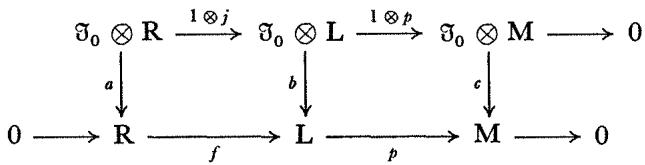
\includegraphics[keepaspectratio]{images/part003_24c814e1.jpg}}

where \(j\) is the canonical injection, \(a, b, c\) deriving from the canonical injection \(\mathfrak{I}_0 \to \mathbf{A}\) ( \(\S 3\) , no. 4, Proposition 4); it must be shown that \(a\) is surjective. Note that, as \(\mathbf{L}\) is free, \(b\) is injective ( \(\S 3\) , no. 7, Corollary 6 to Proposition 7) and \(c\) is injective by hypothesis. Then let \(t\) be an element of \(\mathbf{R}\) and \(t\) its class in \(\mathbf{R} / \mathfrak{I}_0\mathbf{R}\) ; then there is an exact sequence ( \(\S 3\) , no. 6, Proposition 5 and Corollary 2 to Proposition 6)

\[
\mathrm{R} / \mathfrak {I} _ {0} \mathrm{R} \xrightarrow {\jmath} \mathrm{L} / \mathfrak {I} _ {0} \mathrm{L} \xrightarrow {\bar {p}} \mathrm{M} / \mathfrak {I} _ {0} \mathrm{M} \longrightarrow 0
\]

where \(j\) and \(\bar{p}\) derive from \(j\) and \(p\) when passing to the quotients and \(\bar{p}\) is by hypothesis a bijection; then \(\bar{j}(t) = 0\) , in other words \(j(t) \in \mathfrak{I}_0\mathbf{L}\) . Then there is an element \(z \in \mathfrak{I}_0 \otimes \mathbf{L}\) such that \(j(t) = b(z)\) ; as \(p(b(z)) = 0\) , \(c((1 \otimes p)(z)) = 0\) and, as \(c\) is injective, \((1 \otimes p)(z) = 0\) . In other words, \(z\) is the image of an element \(t' \in \mathfrak{I}_0 \otimes \mathbf{R}\) under \(1 \otimes j\) and then \(j(a(t')) = b(z) = j(t)\) ; as \(j\) is injective, this implies \(t = a(t')\) .

We shall show later (Commutative Algebra, II, § 3, no. 2, Proposition 5) how this proposition can be extended to non-graded modules.

Lemma 1. For a commutative group \(\Delta\) to be such that there exists on \(\Delta\) a total ordering compatible with the group structure of \(\Delta\) , it is necessary and sufficient that \(\Delta\) be torsion-free.

If there exists such an order structure on \(\Delta\) and if \(\lambda > 0\) , then \(\lambda + \mu > 0\) for all \(\mu \geqslant 0\) and in particular, by induction on the integer \(n > 0\) , \(n.\lambda > 0\) , which proves that \(\Delta\) is torsion-free (since every element \(\neq 0\) of \(\Delta\) is either \(>0\) or \(< 0\) ). Conversely, if \(\Delta\) is torsion-free, \(\Delta\) is a sub- \(\mathbf{Z}\) -module of a vector \(\mathbf{Q}\) -space ( \(\S 7\) , no. 10, Corollary 1 to Proposition 26) which may be assumed of the form \(\mathbf{Q}^{(I)}\) ; if I is given a well-ordering (Set Theory, III, \(\S 2\) , no. 3, Theorem 1) and \(\mathbf{Q}\) its usual ordering, the set \(\mathbf{Q}^{(I)}\) with the lexicographical ordering is totally ordered (Set Theory, III, \(\S 2\) , no. 6); it is immediate that this ordering is compatible with the additive group structure of \(\mathbf{Q}^{(I)}\) .

PROPOSITION 8. Let \(\Delta\) be a torsion-free commutative group and A a graded ring of type \(\Delta\) . If the product in A of two homogeneous elements \(\neq 0\) is \(\neq 0\) , the ring A has no divisor of 0.

Let \(\Delta\) be given a total ordering compatible with its group structure (Lemma

\begin{enumerate}
\def\labelenumi{\arabic{enumi})}
\tightlist
\item
  and let \(x = \sum_{\lambda \in \Delta} x_{\lambda}, y = \sum_{\lambda \in \Delta} y_{\lambda}\) be two non-zero elements of A ( \(x_{\lambda}\) and \(y_{\lambda}\) being homogeneous of degree \(\lambda\) for all \(\lambda \in \Delta\) ); let \(\alpha\) (resp. \(\beta\) ) be the greatest of the elements \(\lambda \in \Delta\) such that \(x_{\lambda} \neq 0\) (resp. \(y_{\lambda} \neq 0\) ); it is immediate that if \(\lambda \neq \alpha\) or \(\mu \neq \beta\) , either \(x_{\lambda}y_{\mu} = 0\) or \(\deg(x_{\lambda}y_{\mu}) < \alpha + \beta\) ; the homogeneous component of \(xy\) of degree \(\alpha + \beta\) is therefore \(x_{\alpha}y_{\beta}\) , which is non-zero by hypothesis; whence \(xy \neq 0\) .
\end{enumerate}

\subsection{GRADED TENSOR PRODUCT OF GRADED MODULES}

Let \(\Delta\) be a commutative monoid with its identity element denoted by 0, A a graded ring of type \(\Delta\) and M (resp. N) a graded right (resp. left) A-module of type \(\Delta\) . Let \((\mathbf{A}_{\lambda})\) (resp. \((\mathbf{M}_{\lambda}), (\mathbf{N}_{\lambda}))\) be the graduation of A (resp. M, N); the tensor product \(\mathbf{M} \otimes_{\mathbf{Z}} \mathbf{N}\) of the Z-modules M and N is the direct sum of the \(\mathbf{M}_{\lambda} \otimes_{\mathbf{Z}} \mathbf{N}_{\mu}\) (§ 3, no. 7, Proposition 7) and hence the latter form a bigraduation of types \(\Delta, \Delta\) on this Z-module. Consider on M \(\otimes_{\mathbf{Z}} \mathbf{N}\) the total graduation of type \(\Delta\) associated with this bigraduation (no. 1, Example 4); it consists of the sub-Z-modules \(\mathrm{P}_{\lambda} = \sum_{\mu + v = \lambda} (\mathrm{M}_{\mu} \otimes_{\mathbf{z}} \mathrm{N}_{v})\) . It is known that the Z-module M \(\otimes_{\mathbf{A}} \mathbf{N}\) is the quotient of M \(\otimes_{\mathbf{Z}} \mathbf{N}\) by the sub-Z-module Q generated by the elements \((xa) \otimes y - x \otimes (ay)\) , where \(x \in \mathbf{M}, y \in \mathbf{N}\) and \(a \in \mathbf{A}\) (§ 3, no. 1); if, for all \(\lambda \in \Delta\) , \(x_{\lambda}, y_{\lambda}, a_{\lambda}\) are the homogeneous components of degree \(\lambda\) of \(x, y, a\) respectively, clearly \((xa) \otimes y - x \otimes (zy)\) is the sum of the homogeneous elements \((x_{\lambda}a_{v}) \otimes y_{\mu} - x_{\lambda} \otimes (a_{v}y_{\mu})\) , in other words Q is a graded sub-Z-module of M \(\otimes_{\mathbf{Z}} \mathbf{N}\) (no. 3, Proposition 2) and the quotient

\[
\mathbf {M} \otimes_ {\mathbf {A}} \mathbf {N} = (\mathbf {M} \otimes_ {\mathbf {Z}} \mathbf {N}) / \mathbf {Q}
\]

therefore has canonically a graded Z-module structure of type \(\Delta\) (no. 3). Moreover (no. 3, Proposition 5), the centre C of A is a graded subring of A; the graduation which we have just defined on M \(\otimes_{\mathbf{A}} \mathbf{N}\) is compatible with its module structure over the graded ring C. For M \(\otimes_{\mathbf{Z}} \mathbf{N}\) has canonically two C-module structures, for which respectively \(c(x \otimes y) = (xc) \otimes y\) and \((x \otimes y)c = x \otimes (cy)\) for \(x \in \mathbf{M}, y \in \mathbf{N}, c \in \mathbf{C}\) ( \(\S 3\) , no. 3); if \(x \in \mathbf{M}_{\lambda}, y \in \mathbf{N}_{\mu}, c \in \mathbf{C} \cap \mathbf{A}_{\nu}\) , the two elements \(c(x \otimes y)\) and \((x \otimes y)c\) belong to (M \(\otimes_{\mathbf{Z}} \mathbf{N})_{\lambda + \mu + \nu}\) and their difference belongs to Q and hence their common image in M \(\otimes_{\mathbf{A}} \mathbf{N}\) belongs to (M \(\otimes_{\mathbf{A}} \mathbf{N})_{\lambda + \mu + \nu}\) , which establishes our assertion. When we speak of M \(\otimes_{\mathbf{A}} \mathbf{N}\) as a graded C-module, we always mean with the structure thus defined, unless otherwise mentioned. Note that (M \(\otimes_{\mathbf{A}} \mathbf{N})_{\lambda}\) can be defined as the additive group of M \(\otimes_{\mathbf{A}} \mathbf{N}\) generated by the \(x_{\mu} \otimes y_{\nu}\) , where \(x_{\mu} \in \mathbf{M}_{\mu}, y_{\nu} \in \mathbf{N}_{\nu}\) and \(\mu + \nu = \lambda\) .

Let \(\mathbf{M}'\) (resp. \(\mathbf{N}'\) ) be another graded right (resp. left) A-module and \(u: \mathbf{M} \to \mathbf{M}', v: \mathbf{N} \to \mathbf{N}'\) graded homomorphisms of respective degrees \(\alpha\) and \(\beta\) . Then it follows immediately from the above remark that \(u \otimes v\) is a graded (C-module) homomorphism of degree \(\alpha + \beta\) .

When A is commutative, a graduation (compatible with the A-module structure) is similarly defined on the tensor product of any finite number of graded A-modules; it is moreover immediate that the associativity isomorphisms such as \((\mathbf{M} \otimes \mathbf{N}) \otimes \mathbf{P} \to \mathbf{M} \otimes (\mathbf{N} \otimes \mathbf{P})\) (§ 3, no. 8, Proposition 8) are isomorphisms of graded modules.

Remark. When A has the trivial graduation (no. 1, Example 1), \((\mathbf{M} \otimes_{\mathbf{A}} \mathbf{N})_{\lambda}\) is then simply the direct sum of the sub-Y-modules \(\mathbf{M}_{\mu} \otimes_{\mathbf{A}} \mathbf{N}_{\nu}\) of \(\mathbf{M} \otimes_{\mathbf{A}} \mathbf{N}\) such that \(\mu + \nu = \lambda\) .

Let M (resp. N) be a graded right (resp. left) A-module of type \(\Delta\) , P a graded Z-module of type \(\Delta\) and let f be a Z-bilinear mapping of \(M \times N\) into P satisfying condition (1) of §3, no. 1, and such moreover that

\[
f (x _ {\lambda}, y _ {\mu}) \in \mathrm{P} _ {\lambda + \mu} \quad \text { for } x _ {\lambda} \in \mathrm{M} _ {\lambda}, y _ {\mu} \in \mathrm{N} _ {\mu}, \lambda , \mu \text { in } \Delta .
\]

Then \(f(x, y) = g(x \otimes y)\) , where \(g: \mathbf{M} \otimes_{\mathbf{A}} \mathbf{N} \to \mathbf{P}\) is a \(\mathbf{Z}\) -linear mapping (§ 3, no. 1, Proposition 1) and it follows from the above condition that \(g\) is a graded \(\mathbf{Z}\) -module homomorphism of degree 0.

Let B be another graded ring of type \(\Delta\) and \(\rho: A \to B\) a homomorphism of graded rings (no. 2); then \(\rho_*(B_d)\) is a graded right A-module of type \(\Delta\) . If E is a graded left A-module of type \(\Delta\) and \(\rho^*(B_d) \otimes_A E\) is given the graded Z-module structure of type \(\Delta\) defined above, the canonical left B-module structure ( \(\S\) 5, no. 1) is compatible with the graduation of

\[
\mathbf {E} _ {(\mathbf {B})} = \rho^ {*} (\mathbf {E}) = \rho_ {*} (\mathbf {B} _ {d}) \otimes_ {\mathbf {A}} \mathbf {E}.
\]

The graded B-module thus obtained is said to be obtained by extending the ring of scalars to B by means of \(\rho\) and when we speak of \(\mathrm{E}_{(\mathrm{B})}\) or \(\rho^{*}(\mathrm{E})\) as a graded B-module, we always mean this structure, unless otherwise mentioned.

\subsection{GRADED MODULES OF GRADED HOMOMORPHISMS}

We suppose in this no. that the monoid \(\Delta\) is a group. Let A be a graded ring of type \(\Delta\) and M, N two graded left (for example) A-modules of type \(\Delta\) . Let H \(_{\lambda}\) denote the additive group of graded homomorphisms of degree \(\lambda\) of M into N (no. 2); in the additive group Hom \(_{A}\) (M, N) of all homomorphisms of M into N (with the non-graded A-module structures) the sum (for \(\lambda \in \Delta\) ) of the H \(_{\lambda}\) is direct. For, if there is a relation \(\sum_{\lambda} u_{\lambda} = 0\) with \(u_{\lambda} \in \mathrm{H}_{\lambda}\) for all \(\lambda\) , it follows that \(\sum_{\lambda} u_{\lambda}(x_{\mu}) = 0\) for all \(\mu\) and all \(x_{\mu} \in \mathrm{M}_{\mu}\) . As the elements of \(\Delta\) are cancellable, \(u_{\lambda}(x_{\mu})\) is the homogeneous component of \(\sum_{\lambda} u_{\lambda}(x_{\mu})\) of degree \(\lambda + \mu\) ; hence \(u_{\lambda}(x_{\mu}) = 0\) for every ordered pair ( \(\mu, \lambda\) ) and every \(x_{\mu} \in \mathrm{M}_{\mu}\) , which implies \(u_{\lambda} = 0\) for all \(\lambda \in \Delta\) . We shall denote (in this paragraph) by Homgr \(_{A}\) (M, N) the additive subgroup of Hom \(_{A}\) (M, N) the sum of the H \(_{\lambda}\) and we shall call it the additive group of graded A-module homomorphisms of M into N. Let C be the centre of A, which is a graded subring (no. 3, Corollary to Proposition 5); for the canonical C-module structure on \(\mathrm{Hom}_{\mathbf{A}}(\mathbf{M},\mathbf{N})\) (§ 1, no. 14, Remark 1), \(\mathrm{Homgr}_{\mathbf{A}}(\mathbf{M},\mathbf{N})\) is a submodule and the graduation \((\mathbf{H}_{\lambda})\) is compatible with the C-module structure: for, if \(c_{\nu}\in \mathbf{C}\cap \mathbf{A}_{\nu}\) , \(x_{\mu}\in \mathbf{N}_{\mu}\) and \(u_{\lambda}\in \mathbf{H}_{\lambda}\) , then by definition \((c_{\nu}u_{\lambda})(x_{\mu}) = c_{\nu}.u_{\lambda}(x_{\mu})\subset \mathbf{N}_{\lambda +\mu +\nu}\) and hence \(c_{\nu}u_{\lambda}\in \mathbf{H}_{\lambda +\nu}\) .

Let \(\mathbf{M}'\) and \(\mathbf{N}'\) be two graded left A-modules of type \(\Delta\) and \(u':\mathbf{M}'\to\mathbf{M}\) , \(v':\mathbf{N}\to\mathbf{N}'\) graded homomorphisms of respective degrees \(\alpha\) and \(\beta\) . Then it is immediate that \(\operatorname{Hom}(u',v')\colon w\mapsto v'\circ w\circ u'\) maps \(\operatorname{Homgr}_{\mathbf{A}}(\mathbf{M},\mathbf{N})\) into \(\operatorname{Homgr}_{\mathbf{A}}(\mathbf{M}',\mathbf{N}')\) and that its restriction to \(\operatorname{Homgr}_{\mathbf{A}}(\mathbf{M},\mathbf{N})\) is a graded homomorphism into \(\operatorname{Homgr}_{\mathbf{A}}(\mathbf{M}',\mathbf{N}')\) of degree \(\alpha+\beta\) .

In particular \(\operatorname{Homgr}_{\mathbf{A}}(\mathbf{M}, \mathbf{M})\) is a graded subring of \(\operatorname{End}_{\mathbf{A}}(\mathbf{M})\) , which is denoted by \(\operatorname{Endgr}_{\mathbf{A}}(\mathbf{M})\) .

Remark. If M and N are graded left A-modules, \(\operatorname{Homgr}_{\mathbf{A}}(\mathbf{M}, \mathbf{N})\) is in general distinct from \(\operatorname{Hom}_{\mathbf{A}}(\mathbf{M}, \mathbf{N})\) . However these two sets are equal when M is a finitely generated A-module. For M is then generated by a finite number of homogeneous elements \(x_{i}\) ( \(1 \leqslant i \leqslant n\) ); let \(d(i)\) be the degree of \(x_{i}\) ; let \(u \in \operatorname{Hom}_{\mathbf{A}}(\mathbf{M}, \mathbf{N})\) and for all \(\lambda \in \Delta\) let \(z_{i,\lambda}\) denote the homogeneous component of \(u(x_{i})\) of degree \(\lambda + d(i)\) . We show that there exists a homomorphism \(u_{\lambda}: \mathbf{M} \to \mathbf{N}\) such that \(u_{\lambda}(x_{i}) = z_{i,\lambda}\) for all \(i\) . It suffices to prove that if \(\sum_{i} a_{i} x_{i} = 0\) with \(a_{i} \in \mathbf{A}\) for \(1 \leqslant i \leqslant n\) , then \(\sum_{i} a_{i} z_{i,\lambda} = 0\) for all \(\lambda \in \Delta\) (§ 1, no. 7, Remark). It can be assumed that each \(a_{i}\) is homogeneous of degree \(d'(i)\) such that \(d(i) + d'(i) = \mu\) for all \(i\) (no. 3, Remark 1); then \(\sum_{i} a_{i} u(x_{i}) = 0\) ; taking the homogeneous component of degree \(\lambda + \mu\) on the left-hand side, we obtain \(\sum_{i} a_{i} z_{i,\lambda} = 0\) , whence the existence of the homomorphism \(u_{\lambda}\) ; clearly moreover \(u_{\lambda}\) is graded of degree \(\lambda\) . Finally, \(u_{\lambda} = 0\) except for a finite number of values of \(\lambda\) , and \(u = \sum_{\lambda} u_{\lambda}\) by definition, which proves our assertion.

In particular, \(\operatorname{Homgr}_{\mathbf{A}}(\mathbf{A}_s, \mathbf{M}) = \operatorname{Hom}_{\mathbf{A}}(\mathbf{A}_s, \mathbf{M})\) for every graded left A-module M; moreover \(\operatorname{Hom}_{\mathbf{A}}(\mathbf{A}_s, \mathbf{M})\) has a graded left A-module structure (and not just a graded C-module structure), and it is immediate that with this structure the canonical mapping of M into \(\operatorname{Hom}_{\mathbf{A}}(\mathbf{A}_s, \mathbf{M})\) ( \(\S 1\) , no. 14, Remark 2) is a graded A-module isomorphism.

Similarly, \(\operatorname{Homgr}_{\mathbf{A}}(\mathbf{M}, \mathbf{A}_s)\) has a graded right A-module structure (and not only a graded C-module structure); it is called the graded dual of the graded A-module M and is denoted by \(\mathbf{M}^{*\mathbf{gr}}\) , or simply \(\mathbf{M}^*\) when no confusion results. If \(u: \mathbf{M} \to \mathbf{N}\) is a graded homomorphism of degree \(\delta\) , it follows from the above that the restriction to \(\mathbf{N}^{*\mathbf{gr}}\) of \(^t u = \operatorname{Hom}(u, 1_{\mathbf{A}_s})\) is a graded homomorphism of the graded dual \(\mathbf{N}^{*\mathbf{gr}}\) into the graded dual \(\mathbf{M}^{*\mathbf{gr}}\) , of degree \(\delta\) , called the graded transpose of \(u\) .

We sometimes consider on the graded dual \(M^{*gr}\) the graduation derived from the above with the aid of the isomorphism \(\lambda\mapsto-\lambda\) of \(\Delta\) (no. 1, Example 2) so that the homogeneous elements of degree \(\lambda\) in \(M^{*gr}\) are the graded linear forms of degree \(-\lambda\) on M (when A has the trivial graduation, these are the zero linear forms of the \(M_{\mu}\) of index \(\mu\neq\lambda\) ). Then, if \(u:M\to N\) is a graded homomorphism of degree \(\delta\) , \(u'\) becomes a graded homomorphism of degree \(-\delta\) .

Suppose A is commutative and graded of type \(\Delta\) and let M, N, P, Q be four graded A-modules of type \(\Delta\) . Then there are canonical graded homomorphisms of degree 0

\begin{enumerate}
\def\labelenumi{(\arabic{enumi})}
\setcounter{enumi}{2}
\tightlist
\item
\end{enumerate}

\[
\operatorname{Homgr} _ {\mathbf {A}} (\mathbf {M}, \operatorname{Homgr} _ {\mathbf {A}} (\mathbf {N}, \mathbf {P})) \rightarrow \operatorname{Homgr} _ {\mathbf {A}} (\mathbf {M} \otimes_ {\mathbf {A}} \mathbf {N}, \mathbf {P})\tag{4}
\]

\[
\operatorname{Homgr} _ {\mathbf {A}} (\mathbf {M}, \mathbf {N}) \otimes_ {\mathbf {A}} \mathrm{P} \rightarrow \operatorname{Homgr} _ {\mathbf {A}} (\mathbf {M}, \mathbf {N} \otimes_ {\mathbf {A}} \mathrm{P})
\]

\[
\operatorname{Homgr} _ {\mathbf {A}} (\mathbf {M}, \mathbf {P}) \otimes_ {\mathbf {A}} \operatorname{Homgr} _ {\mathbf {A}} (\mathbf {N}, \mathbf {Q}) \rightarrow \operatorname{Homgr} _ {\mathbf {A}} (\mathbf {M} \otimes_ {\mathbf {A}} \mathbf {N}, \mathbf {P} \otimes_ {\mathbf {A}} \mathbf {Q}) \tag {5}
\]

(the tensor products being given the graduations defined in no. 5) obtained by restricting the canonical homomorphisms defined in §4, nos. 1, 2 and 4; for, if \(u: \mathbf{M} \to \operatorname{Homgr}_{\mathbf{A}}(\mathbf{N}, \mathbf{P})\) is graded of degree \(\delta\) , then, for all \(x \in \mathbf{M}_{\lambda}\) , \(u(x)\) is a graded homomorphism \(\mathbf{N} \to \mathbf{P}\) of degree \(\delta + \lambda\) and hence, for \(y \in \mathbf{N}_{\mu}\) , \(u(x)(y) \in \mathbf{P}_{\delta + \lambda + \mu}\) ; if \(v: \mathbf{M} \otimes_{\mathbf{A}} \mathbf{N} \to \mathbf{P}\) corresponds canonically to \(u\) , it is then seen that \(v\) is a graded homomorphisms of degree \(\delta\) , whence our assertion concerning (3); moreover it is seen that this homomorphism is bijective. The argument is similar for (4) and (5).

If in particular \(\mathbf{P} = \mathbf{Q} = \mathbf{A}\) in (5), then there is a canonical graded homomorphism of degree 0

\[
\mathbf {M} ^ {* \mathrm{gr}} \otimes_ {\mathbf {A}} \mathbf {N} ^ {* \mathrm{gr}} \rightarrow (\mathbf {M} \otimes_ {\mathbf {A}} \mathbf {N}) ^ {* \mathrm{gr}}.\tag{6}
\]

\BourbakiAppendixSection{Pseudomodules}

\subsection{ADJUNCTION OF A UNIT ELEMENT TO A PSEUDO-RING}

Let A be a pseudo-ring (I, § 8, no. 1). On the set \(\mathbf{A}' = \mathbf{Z} \times \mathbf{A}\) we define the following laws of composition:

\[
\left\{ \begin{array}{l} (m, a) + (n, b) = (m + n, a + b) \\ (m, a) (n, b) = (m n, m b + n a + a b). \end{array} \right.\tag{1}
\]

It is immediately verified that A' with these two laws of composition is a ring in which the element \((1,0)\) is the unit element. The set \(\{0\} \times A\) is a two-sided ideal of A' and \(\iota: x \mapsto (0, x)\) is an isomorphism of the pseudo-ring A onto the sub-pseudo-ring \(\{0\} \times A\) by means of which A and \(\{0\} \times A\) are identified. A' is called the ring derived from the pseudo-ring A by adjoining a unit element.

If A already has an identity element \(\varepsilon\) , the element \(e = (0, \varepsilon)\) of \(\mathbf{A}'\) is an idempotent belonging to the centre of \(\mathbf{A}'\) and such that

\[
\mathrm{A} = e \mathrm{A} ^ {\prime} = \mathrm{A} ^ {\prime} e.
\]

Then \((e\mathbf{A}', (1 - e)\mathbf{A}')\) is a direct decomposition (I, § 8, no. 11) of \(\mathbf{A}'\) and the ring \((1 - e)\mathbf{A}'\) is isomorphic to \(\mathbf{Z}\) .

\subsection{PSEUDOMODULES}

Given a pseudo-ring A with or without a unit element, a left pseudomodule over A is a commutative group E (written additively) admitting A as set of operators and satisfying axioms \((\mathbf{M}_{\mathrm{I}})\) , \((\mathbf{M}_{\mathrm{II}})\) and \((\mathbf{M}_{\mathrm{III}})\) of §1, no. 1, Definition 1. Right pseudomodules over A are defined similarly.

Let \(A'\) be the ring obtained by adjoining a unit element to A. If E is a left pseudomodule over A, a left \(A'\) -module structure on E is associated with it by writing, for all \(x \in E\) and every element \((n, a) \in A'\) ,

\[
(n, a). x = n x + a x.\tag{2}
\]

Axioms \((\mathbf{M}_{\mathrm{I}})\) to \((\mathbf{M}_{\mathrm{IV}})\) of § 1, no. 1, Definition 1 are immediately verified; moreover, by restricting the set of operators of this module structure to \(\{0\} \times A\) (identified with A), we obtain on E the pseudomodule structure given initially.

For a subset M of E to be a subgroup with operators of the pseudomodule E (in which case the induced structure is obviously also a left pseudomodule structure over A), it is necessary and sufficient that M be a submodule of the associated A'-module E and this sub-A'-module is associated with the pseudomodule M. Moreover, the quotient A'-module E/M is then associated with the quotient group with operators E/M, which is obviously a pseudomodule over A.

If E, F are two pseudomodules over A, the homomorphisms \(E \rightarrow F\) of groups with operators are identical with the A'-linear mappings \(E \rightarrow F\) of the A'-modules associated respectively with the pseudomodules E and F. If \((\mathbf{E}_{t})_{t \in I}\) is a family of pseudomodules over A, the groups with operators \(\prod_{i\in I}E\) and \(\bigoplus_{i\in I}E_{i}\) are pseudomodules over A and the associated A'-modules are respectively the product and direct sum of the associated A'-modules \(E_{i}\) . There are analogous results for inverse and direct limits of pseudomodules. The theory of pseudomodules over A can thus be entirely reduced to that of A'-modules.

\BourbakiExercisesHeading
